%
% TTÜ Style Thesis template for LaTeX
%
% Public Version 1.1
% 2019 Adjusted by Frank Korving for his TTÜ Bachelor Thesis
% With Contributions from Tarvo Reinpalu, Priit Ruberg and Sander Arnus
%
% Public version 1.0
% 2010 - 2013 Thijs Nugteren and Joos Buijs for TU/e Master Thesis
%
% THIS IS THE MAIN FILE (i.e. compile this file, compiling the others directly won't work)
%
\documentclass[12pt, a4paper]{report}

% all the other includes etc. are done in the thesis.sty file.
\usepackage{thesis}

%
% These commands need to be defined in order to produce a correct and personalized document
%
\newcommand{\doctitle}{Choosing and Implementing Continuous Integration: the Case of Certidude}
\newcommand{\docsubtitle}{Diploma Thesis}

\newcommand{\me}{Frank Korving}
\newcommand{\studentcode}{176209IDCR}
\newcommand{\university}{TALLINN UNIVERSITY OF TECHNOLOGY}
\newcommand{\school}{School of Information Technology}
\newcommand{\department}{Information Technology College}
\newcommand{\supervisor}{Lauri Võsandi}
\newcommand{\supervisortitle}{MSc}
\newcommand{\cosupervisor}{Kaido Kikkas}
\newcommand{\cosupervisortitle}{PhD}
\newcommand{\keywords}{DevOps, CI/CD, Continuous Integration, Docker, Jenkins, GitlabCI, CircleCI, TravisCI, TeamCity}
\newcommand{\version}{0.1 version}
\newcommand{\monthYear}{April 2019}
\newcommand{\Year}{2019}
\newcommand{\signatureDate}{May 20, 2019}

\author{\me}

%
% PDF settings
%
\hypersetup
{
    pdfauthor={\me},
    pdfsubject={\doctitle},
    pdfkeywords={\keywords}
}

\begin{document}
\pagenumbering{roman}
\begin{titlepage}
\headheight = 57pt
\footskip = 5pt
\headsep = 0pt

\centering
\textsc{\begin{Large}
\university\\
\end{Large} }
\school\\
\department\\

\vspace*{7 cm}

\begin{center}

\me \quad \studentcode\\
\begin{Large}
\textsc{\textbf{\doctitle}}\\
\end{Large}
\docsubtitle\\
\end{center}

\begin{flushright}
\textbf{Technical Supervisor}\\ \supervisor\\\supervisortitle\\
\textbf{Academic Supervisor}\\\cosupervisor\\\cosupervisortitle
\end{flushright}

\vfill

Tallinn \Year
\end{titlepage}

\normalsize

\chapter*{\centerline{Author's declaration of originality}}\label{chapter:declaration}
\hfill \\
I hereby certify that I am the sole author of this thesis. All the used materials, references
to the literature and the work of others have been referred to. This thesis has not been
presented for examination anywhere else.

\vskip1in
\begin{flushleft}
\begin{tabular}{p{2.0cm}p{6.0cm}p{4.0cm}}
  Author: & \me & ......................................\\
  && \hfill(signature)\\
  Date: & \signatureDate &\\
  \\
  \\

% Uncomment the following to add supervisor declaration
%  \multicolumn{3}{l}{The thesis adheres to all specified requirements}\\
%  \hfill \\
%  Supervisor: & \supervisor & ......................................\\
%  && \hfill(signature)\\
%  Date: & \signatureDate &\\


\end{tabular}
\end{flushleft}

\chapter*{\centerline{Annotatsioon}}\label{chapter:abstract-eesti}
Certidude on Eesti päritoluga, avatud lähtekoodiga projekt, mille
eesmärgiks on muuta igapäevane VPN-sertifikaatide haldamine 
süsteemiadministraatorite jaoks võimalikult lihtsaks. Nagu
mitmetel teistel tarkvaraprojektidel, on Certidude’il testimisprotseduur,
mis suurendab koodi kvaliteedikindlust ja tagab juurutamisel soovitud
funktsionaalsuse. 

Certidude'i sihiks on kasutada arenduses pidevintegratsiooni  ja
-valmidust (CI/CD), et automatiseerida integratsiooniteste ja teisi
tunnustatud arendustavasid. Praeguse töövahendi piirangud on siiski
vähendanud nende kasulikkust Certidude’i jaoks ja tinginud selle
asendamise vajaduse.

Käesolevas lõputöös uuritakse levinumaid CI/CD serveri komponente ja
lahendusi, töötatakse välja testimisrakendus ja võrreldakse selle abil
viit levinud CI/CD serverilahendust. Gitlab CI vastas defineeritud
nõuetele kõige paremini, mistõttu Certidude’is võeti kasutusele see
töövahend.

Olemasolev Certidude’i testimisprotseduur vajab veel palju täiustamist,
mistõttu on koostatud ettepanekute nimekiri, mida saab kasutada arenduse
tegevuskavana. Lisaks võib seda lõpu tööd käsitleda lühikese juhendina
CI/CD maailma. Pidevintegratsioonist ja sellega seotud mõistetest
antakse ülevaade peatükkides \ref{chapter:introduction} ja \ref{chapter:concepts}, peatükis \ref{chapter:analysis} asub võrdlev analüüs ja
peatükis \ref{chapter:implementation} realisatsioon. Arenduse lisafailid võib leida  aadressilt 
\url{https://github.com/Korving-F/thesis-cicd-examples}.

Lõputöö on kirjutatud inglise keeles ning sisaldab teksti 34 leheküljel, 5 peatükki, 20 joonist, 2 tabelit.
\pagebreak

\chapter*{\centerline{Abstract}}\label{chapter:abstract}
Certidude is an Estonia-based, open source project aiming to make VPN certificate 
management as easy as possible for everyday system administrators. Like many other software projects,
Certidude has a test-suite that should increase confidence in code quality and ensure the presence of desired
functionality when deployed. Certidude already tries to make use of development practices like 
Continuous Integration and Delivery to automate integration tests and other development best practices, 
but limitations of the current tool have dulled their usefulness for Certidude and created the need 
for a replacement.

During this research common CI/CD server components and integrations were explored and discussed,
a test application was developed and
a comparative analysis was performed between five popular CI/CD server implementations based on that
application. Gitlab CI revealed itself to be the best fit according to defined requirements so a replacement
pipeline for Certidude was implemented in that tool. 

The current test-suite of Certidude still needs a lot of work, so in addition a list of "\textit{future work}"
suggestions was compiled which can be used as a development road map. Additionally this thesis can be considered
a short guide into the world of CI/CD. 

See Chapters \ref{chapter:introduction} and \ref{chapter:concepts} for an overview of Continuous Integration and related concepts, Chapter \ref{chapter:analysis} for the comparative analysis and Chapter \ref{chapter:implementation} for the implementation. The developed test application and pipeline files can be found here: \url{https://github.com/Korving-F/thesis-cicd-examples}

The thesis is in English and contains 34 pages of text, 5 chapters, 20 figures, 2 tables.
\pagebreak

\chapter*{\centerline{List of abbreviations and terms}}\label{chapter:terms}
\begin{longtable}{p{3cm}p{10cm}}
AD&Active Directory\\
API&Application Programming Interface\\
CA&Certificate Authority\\
Chroot&Change Root\\
CI/CD&Continuous Integration / Continuous Delivery\\
CLI&Command Line Interface\\
COW&Copy On Write\\
CPU&Central Processing Unit\\
CRL&Certificate Revocation List\\
CSR&Certificate Signing Request\\
CVE&Common Vulnerabilities and Exposures\\
DAST&Dynamic Application Security Testing\\
DC&Domain Controller\\
DSL&Domain Specific Language\\
GUI&Graphical user interface\\
HTML&Hypertext Markup Language\\
HTTP(S)&Hyper Text Transfer Protocol (Secure)\\
IDE&Integrated Development Environment\\
IOT&Internet Of Things\\
JSON&JavaScript Object Notation\\
LDAP&Lightweight Directory Access Protocol\\
LXC&Linux Container\\
LXD&Linux Container Daemon\\
NIST&National Institute of Standards and Technology\\
NVD&National Vulnerability Database\\
OCSP&Online Certificate Status Protocol\\
OVAL&Open Vulnerability and Assessment Language\\
OWASP&Open Web Application Security Project\\
PKI&Public Key Infrastructure\\
RPM&Red Hat Package Manager\\
SAST&Static Application Security Testing\\
SCAP&Security Content Automation Protocol\\
SSL&Secure Sockets Layer\\
SQL&Structured Query Language\\
TDD&Test Driven Development\\
TLS&Transport Layer Security\\
UX&User Experience\\
VCS&Version Control System\\
VM&Virtual Machine\\
VPN&Virtual Private Network\\
WAR&Web application ARchive\\
X.509&Certificate Format\\
XCCDF&Extensible Configuration Checklist Description Format\\
XML&Extensible Markup Language\\
YAML&YAML Ain't Markup Language\\
\end{longtable}
\addtocounter{table}{-1} 
\pagebreak

\phantomsection
\setcounter{tocdepth}{2}    % Sets maximum depth of Table Of Contents
\renewcommand{\contentsname}{Table of Contents}
\tableofcontents

\clearpage
\phantomsection
\setcounter{figure}{0}
\addcontentsline{toc}{chapter}{\listfigurename}
\listoffigures

\clearpage
\phantomsection
\addcontentsline{toc}{chapter}{\listtablename}
\listoftables

\chapter{Introduction}\label{chapter:introduction}
\onehalfspacing
\setcounter{page}{0}
\pagenumbering{arabic}   %from here on, start the 'real' page numbering, from 1, with normal digits
Testing often is an integral part of software development processes. When new code gets added to a project, old features and functionality need to be verified, code styles need to be enforced and security scans should reveal any vulnerabilities that may be present. This raises the overall code quality and security of the software under development.
Unfortunately these steps can be quite labor intensive and are therefore sometimes ignored or neglected. This is where CI (Continuous Integration) comes into play and together with CD (Continuous Delivery) will be generically referred to as continuous practices. See Section \ref{sec:continuous-practices} for a more in-depth description of and distinction between these concepts.

%\textit{Continuous Integration} refers to a development practice where developers frequently merge their code in a shared repository which sets off an automated build/test process and verifies the quality of the code submission, its integration with the existing code base and supporting services.\cite{fowler, thoughtworks-ci}
%The main aim of this practice is to automate good code development habits to catch and fix any code bugs as soon as they occur. This raises overall confidence in the code quality of the project.

%\textit{Continuous Delivery} is a term often used as an extension of and in conjunction with Continuous Integration. It adds to CI by dealing with application release automation, among others. This maintains a state where the application under development is always tested and ready to be deployed.\cite{continuous-delivery-2} These combined will be generically referred to as continuous practices.

Implementing continuous practices is done using automation servers which facilitate the build and test processes of the application. They are henceforth interchangeably referred to as either CI servers or CI/CD servers since they often are capable of automating tasks that range the scope of both concepts. Series of these automated tasks are generally referred to as a \textit{pipelines}.

Certidude is the software project under test and the subject of this work. It is an open-source CA (Certificate Authority) management tool designed to make signing and revocations of certificates easier.\cite{certidude} While Certidude currently already has a CI/CD solution in place (TravisCI) there are some issues that motivate the search for a replacement:
\begin{itemize}
    \item Since this CI/CD solution is cloud based, only a limited amount of resources are available and general control over the CI/CD server is minimal. Many of Certidude's integration tests rely on services that are all currently bootstrapped onto the same machine instead of on dedicated instances (e.g. Virtual Private Network Gateway (VPN), VPN Client, Samba as Domain Controller (DC) for Active Directory (AD) integration tests etc.). Implementing this has proven to be problematic for the current tool.
    \item Support for Ubuntu Xenial (16.04) VMs has only recently started.\cite{travis-os-support} Slow support for newer versions of Operating Systems (OS) could be an issue if the application and its tests can't be properly containerized since compatibility with deployment OS is important.
\end{itemize}

\pagebreak

A number of popular CI/CD server solutions are available, but all come with different features and are continuously being improved upon by their developers. It can be a time consuming task to sift through these solutions and determine which is best suited for the project at hand.

The goal of this work is to perform a comparative analysis of popular CI/CD server implementations and choose the one best suited for Certidude based on a series of determined use cases and requirements. This thesis contributes such an analysis. The aim is to have this tool of choice be implemented, configured and at least meet the minimum requirement of being able to replace the current tool. An additional aim of this work will be to explore and implement some common test and security utilities that can be used in CI/CD pipelines and which are currently not yet implemented. While deploying the code (CD) is considered out of scope, compiling OpenWrt images as a CI task will be explored as well.

A constraint on this work will be the number of CI/CD server implementations under analysis. There are dozens of candidate tools available which potentially could perform some of the needed tasks in one form or another. However, running tests in all of these would be too time consuming. This will also be shortly addressed during the analysis phase in Chapter \ref{chapter:analysis}.

Tests and a practical comparison were based on an application developed for this thesis and for which the various CI/CD servers were installed, configured and implementation-specific pipelines were created. These can be found in Appendices \hyperref[chapter:appendix-travis]{1}, \hyperref[chapter:appendix-jenkins]{2}, \hyperref[chapter:appendix-gitlab]{3}, \hyperref[chapter:appendix-tc]{4} and \hyperref[chapter:appendix-circleci]{5}. A recommendation was given to the main developer of Certidude, \supervisor, after which a choice between the tools was made.

This thesis contributes both a minimum working replacement for the current tool in use and its pipeline configurations as well as an expansion on functionality by the inclusion of multiple static code analysis tasks and an OpenWrt image creation task in the developed pipeline. These and supporting materials can be found in Appendices \hyperref[chapter:appendix-certidude-pipeline]{6}, \hyperref[chapter:appendix-sonar]{7}, \hyperref[chapter:appendix-vbox]{8} and \hyperref[chapter:appendix-openwrt]{9}. In addition a list of "future  work"  suggestions  was compiled in Section \ref{future-work}, which  can  be used  as part of  a  development road map for Certidude.

The author would like to thank the supervisors of this work, \cosupervisor{} and \supervisor, for their ideas, critical feedback and without whom this work would not exist. Many thanks go out as well towards TeamCity, Jenkins, Gitlab, CircleCI and Travis CI for providing access to their tools.

\chapter{Technologies and Concepts}\label{chapter:concepts}
This chapter will take a more in-depth look at CI/CD. Some of the core terms, concepts and technologies commonly used in CI/CD practices will be described and explained. An overview of Certidude will be given as well.

\section{Certidude}
Certidude is an open-source CA management tool mainly designed for VPN gateway operators to make VPN client setups on laptops, desktops and other devices easier.\cite{certidude} Certidude allows for easy signing, revoking and review of (authorized) X.509 certificates and CSRs (Certificate Signing Request) used in establishing VPN tunnels and accessing a company's PKI (Public Key Infrastructure) as a whole. It integrates with authentication protocols like LDAP (Lightweight Directory Access Protocol) and Kerberos and is able to provide CRLs (Certificate Revocation Lists) and OCSP (Online Certificate Status Protocol) responses to querying gateways ensuring the validity of presented certificates. See Figure \ref{fig:certidude} for an overview of Certidude and how it relates to other services.

\begin{figure}[ht]
    \centering
    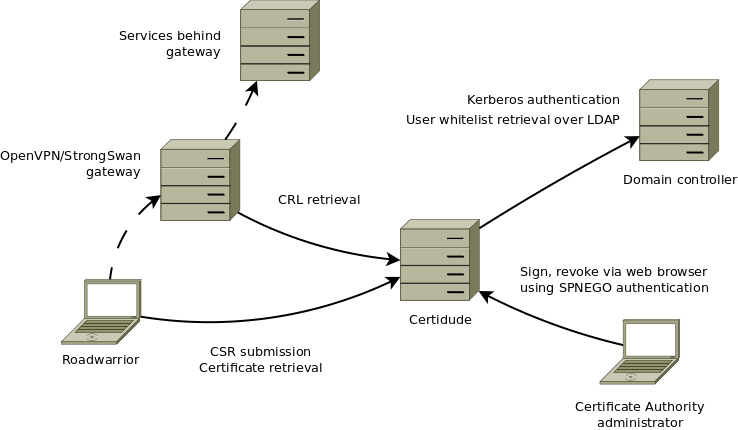
\includegraphics[width=\textwidth]{figures/certidude2.png}
    \caption{\textit{An overview of Certidude and integrated services.}\cite{certidude}}
    \label{fig:certidude}
\end{figure}

\section{Continuous Integration, Delivery, Deployment}\label{sec:continuous-practices}
Continuous practices revolve around using adequate version control systems, integrating code often and fixing code the moment it becomes apparent it has broken. It plays well with other development practices like TDD (Test Driven Development) and refactoring because of their focus on incremental changes and improvements.\cite{ci-duvall} Adhering to these types of best practices allow for companies to frequently and reliably release new features and products, consequently adding business value.\cite{cicd-review}

The generic set of Continuous practices can be subdivided in logical parts. Defining where practicing Continuous Integration, Delivery or Deployment start and stop seems however to be a somewhat hard task to execute since no official consensus exists. The definition for Continuous Integration that seems by far most popular is that of Martin Fowler from his popular "\textit{Continuous Integration}" article:

\textit{"Continuous Integration is a software development practice where members of a team integrate their work frequently, usually each person integrates at least daily - leading to multiple integrations per day. Each integration is verified by an automated build (including test) to detect integration errors as quickly as possible."}\cite{ci-duvall,cicd-review,fowler,cd-casestudy,devops-implementation}

Continuous Delivery generally aims to ensure that an application under development is production-ready at all times and combines Continuous Integration with the \textit{possibility} of deployment automation.\cite{cicd-review,deploymentvdelivery,continuous-delivery} This means that at any time, code present in the shared repository should be deployable and should have passed all tests. Benefits for associated practices have been a reduced deployment risk (less can go wrong with small changes) and more immediate user feedback (develop only useful software).\cite{cicd-review,continuous-delivery}

Continuous Deployment adds to Continuous Delivery by actually automatically deploying code to a production server the moment tests are passed. It's goals seem to overlap with those of Continuous Delivery. The main difference is its push-based approach, as opposed to Continuous Delivery's pull based approach where a later review process determines what actually gets deployed.\cite{cicd-review,deploymentvdelivery,continuous-deployment}

\pagebreak

A lot of tasks and best practices associated with CI/CD allow for them to be automated: automatic unit/integration testing, automatic code quality scans, automatic deployment of code, automatic packaging and automatic reporting on all of the above. Various automated build servers have emerged to make the life of developers and administrators easier and which often allow for many native and 3rd party tool integrations.

The purpose of these integrations and tools are varied. The following use cases are merely a subset:\cite{cicd-review} 
\begin{itemize}
    \item Reduce test and build time 
    \item Increase visibility and awareness on build and test results
    \item Detect violations, flaws and faults
    \item Address security and scalability issues
\end{itemize}

Defining the steps and components these build servers need come with their own associated jargon.\cite{oss-tdd} A high level overview can be seen in Figure \ref{fig:pipeline-overview} which consists of the following building blocks:
\begin{itemize}
    \item \textbf{Job} or \textbf{Task}: a series of sequential instructions (e.g. code checkout through git)
    \item \textbf{Stage}: a collection of jobs that could be executed non-sequentially (e.g. test phase)
    \item \textbf{Pipeline}: a collection of stages that are executed sequentially
\end{itemize}

\begin{figure}[ht]
    \centering
    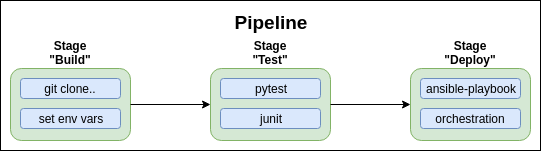
\includegraphics[width=\textwidth]{figures/drawio/pipeline_overview.png}
    \caption{\textit{An overview of CI/CD building blocks}}
    \label{fig:pipeline-overview}
\end{figure}

\pagebreak

Historically these different jobs, stages and pipelines were commonly configured through GUI-based web form submissions and other abstractions which distanced programmers from their build configurations.\cite{intro-pipeline-as-code,jenkins-pipeline} This approach had other problems like being unable to track changes to build configurations, which result in non-reproducible builds and the inability for programmers to change the pipeline that resides on a centralized build server.\cite{what-pipeline-as-code}


The build-as-code approach introduced by TravisCI popularized the idea that the pipeline configuration is part of the same VCS (Version Control System) repository as the software project it is supposed to build and test. On top of that its pipeline configuration was done in a human-readable format through a declarative syntax using YAML files.\cite{what-pipeline-as-code}

Next generation CI/CD build servers introduced the capability to configure pipelines through full programming languages or specialized DSLs (Domain Specific Language) which also became part of the VCS repository. This added complexity to the writing of pipelines but allowed for the setup of more complex pipelines through the use of parameterization, conditional execution and other language constructs as well.\cite{what-pipeline-as-code} Some other advantages could be syntax-highlighting and auto-complete in modern IDEs (Integrated Development Environments). Some examples include:
\begin{itemize}
    \item TeamCity's Kotlin-based DSL as an alternative to their XML format.\cite{teamcity-dsl}
    \item Jenkins's Groovy-based DSL.\cite{jenkins-dsl}
    \item Gomatic through Python.\cite{gomatic-gpl}
\end{itemize}

Currently it is common for declarative pipeline definition syntaxes to include functionality like conditional execution and inheritance as well. These include TravisCI, GitlabCI (both use YAML files) and the previously mentioned Jenkins that also supports a declarative pipeline definition syntax.\cite{jenkins-declarative}

\pagebreak

\section{Pipeline Integrations}
This section will shortly discuss some of the type of tools that are commonly used in CI/CD pipelines. This should help to illustrate the power and flexibility of CI/CD servers, their applicability in the field of Cyber-Security as well as prepare for Chapter \ref{chapter:analysis} and Chapter \ref{chapter:implementation}, where some of these are implemented and/or compared.

Once a CI/CD automation server is present, it opens up the door to define a large amount of pipelines, stages and jobs that utilize a wide variety of native and third-party tools. Figure \ref{fig:deployment-pipeline} shows some of these, including CI servers themselves. Some of these are generic and usable for all programming languages, others are language specific or assume a specific type of application under development. Since Certidude is a Python based application the focus is on those tools that provide support for it, but most if not all type of tools have Python specific analogous implementations or are language independent.

\begin{figure}[ht]
    \centering
    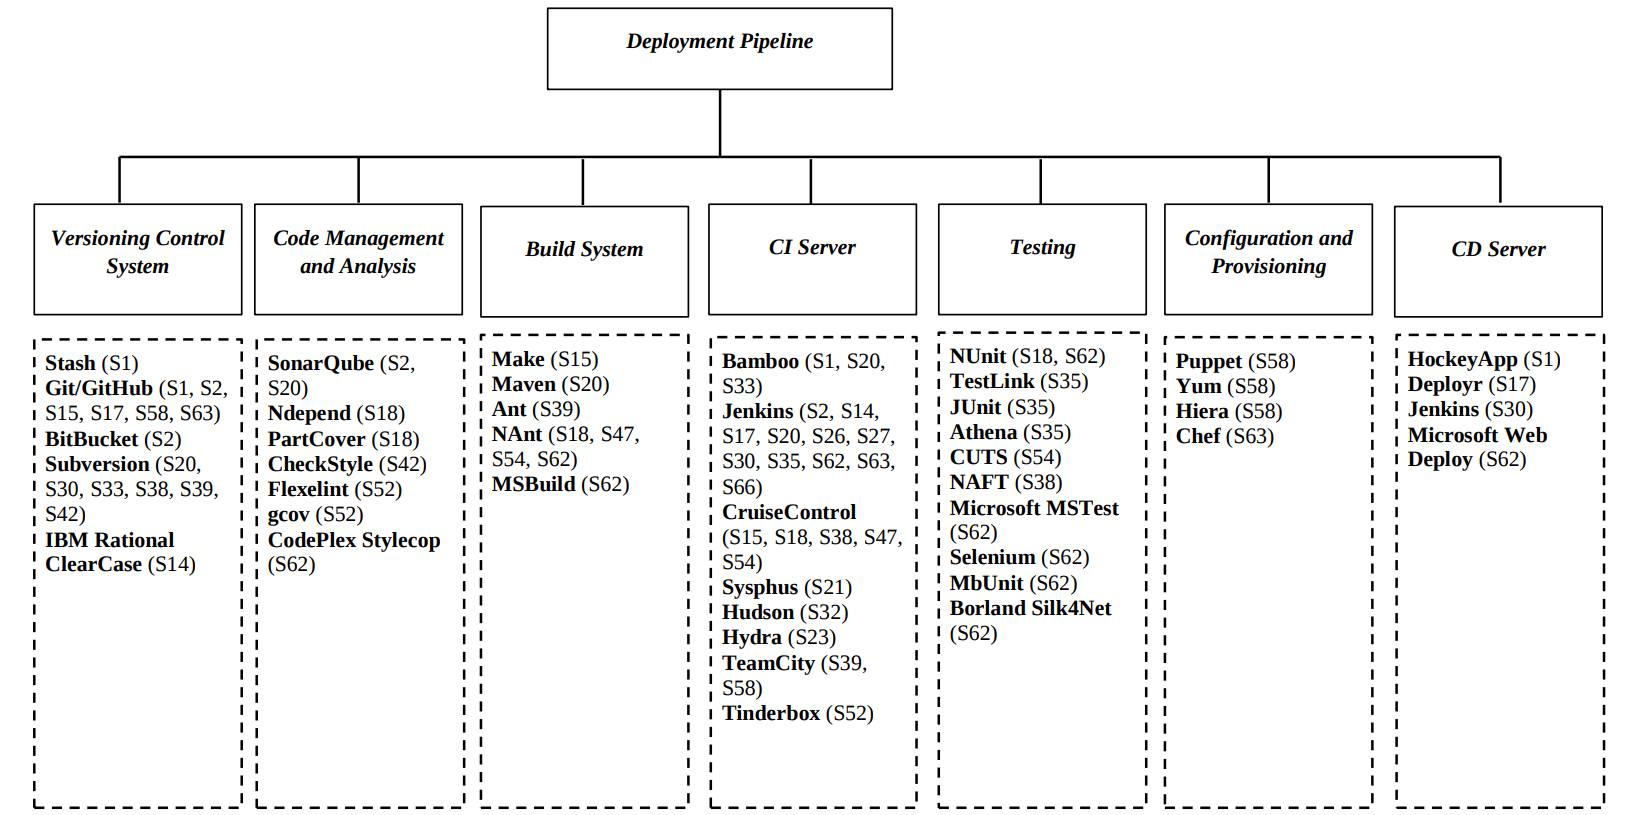
\includegraphics[width=\textwidth]{figures/deployment_pipeline.png}
    \caption{\textit{An overview of tools used in CI/CD pipelines.}\cite{cicd-review}}
    \label{fig:deployment-pipeline}
\end{figure}

\subsection{Build Agent}
As could be seen in Figure \ref{fig:pipeline-overview}, we need to execute some commands and run utilities during our build, test and deploy stages in the pipeline. The question then arises: where are these executed? Some CI/CD servers allow for build agents to be installed on machines which will either listen for incoming requests or fetch user-defined instructions for execution through an API (Application Programming Interface). These can be UNIX machines executing bash scripts but also Windows devices executing PowerShell commands.\cite{gitlab-shell} They capture output of these instructions and feed this and more back to the main CI/CD server. See Figure \ref{fig:cicdserver-agent} for a high-level overview.

\begin{figure}[ht]
    \centering
    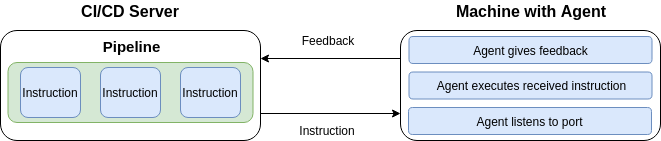
\includegraphics[width=\textwidth]{figures/drawio/cicdserver-agent.png}
    \caption{\textit{High-Level view of a CI/CD server agent interaction}}
    \label{fig:cicdserver-agent}
\end{figure}

While agents can often be installed on any host machine, they are commonly set-up in or setup to control virtualized environments like virtual-machines or containers. This ensures a clean build environment each time the agents receives and runs pipeline instructions. This is important because this allows for dependencies to be more accurately identified, software is tested in the same environment each time tests are run and the test environment can be \textit{exactly} the same as production.

The exact inner workings of virtualization technology is out of scope for this thesis, however it is important to talk about some of their fundamentals, popular implementations and differences.

\subsubsection{VMs} \label{subsec:VMs}
Virtual Machines are emulations of computer systems which provide the same functionality as physical computers. They are generally referred to as \textit{"guests"} while the computing environment within which they are run are referred to as \textit{"hosts"}. Microsoft's documentation describes running a virtual machine as: \textit{"...creating a computer within a computer."}\cite{azure-vm} 

On a typical system the OS's kernel, or supervisor, is the piece of software that is interacting closest with the underlying hardware.
To get things done applications make system calls to the kernel which has higher privileges and in turn grants access to physical resources like memory and the CPU (Central Processing Unit). The kernel of a VM (Virtual Machine) however is presented with virtual resources and its access to hardware is validated and controlled by the host machine. This isolates the host from one, or potentially many VMs running on top of it. To have virtualization capabilities requires what's called a \textit{hypervisor}, also called the supervisor of the supervisor.\cite{virt-dummy,what-is-hypervisor} 

\pagebreak

In practice this can be implemented in software as well as be enabled through special flags in a CPU's architecture instruction set.\cite{virtualbox-virt,hardware-virt} This mechanism of having different levels of privilege is also referred to as ring-protection and is meant to make it harder for common applications, or VMs in this case, to maliciously and/or accidentally crash or corrupt the whole system they are running on.\cite{computerphile-virt}  See Figure \ref{fig:protection-rings} for an overview of protection rings where a hypervisor would run in ring -1.

Virtual Machines are also important because they allow for snapshots, capturing the exact state of a system at a specific point in time and allow for rollback to that state. After a snapshot is made each change to the system is recorded. Rolling back means throwing away those changes.\cite{virtualbox-snap} This enables CI/CD agents to be installed on clean VMs, a snapshot to be created, let these agents execute steps in the build process like installing dependencies, running the code under test, run the tests on that code then report back to the CI/CD server and restore the original state. This level of insight into and control over machine state and code dependencies increases confidence that the code under test will run on production machines as expected.

\begin{figure}[ht]
    \centering
    \includegraphics[width=.5\textwidth]{figures/privilege_rings.png}
    \caption{\textit{Overview of protection rings.}\cite{protection-rings}}
    \label{fig:protection-rings}
\end{figure}

% TODO: Still mention type 1 paravirtualization / type 2 hw-accellerated virtualization through CPU flags / CPU opcodes vm-enter vm-exit..
%       LXD would be a "type 3" linux-only hypervisor.

\subsubsection{Containers}  \label{subsec:containers}
OS-level virtualization, or in its common name "\textit{container}"-technology, is different from traditional VMs and is sometimes described as somewhere between a chroot and a full-blown VM.\cite{lxc} Chroot-environments are a way to isolate processes and applications in a sub-tree of the file system and resembles \textit{installing an OS into your existing OS}.\cite{basic-chroot} This means that one or multiple containers running on a host all share the same kernel with the host instead of having their own. Some popular implementations are BSD-jails\cite{bsd-jail}, LXC\cite{arch-lxc} (Linux Container) and Docker\cite{arch-docker}. Linux based containers (e.g. Docker and LXC) build on top of chroot-environments by using cgroups for resource management \cite{arch-cgroups}, AppArmor / SELinux profiles for security \cite{lxc-intro} and namespaces for isolation.\cite{docker-namespace,evans-container}

\pagebreak

They provide similar capabilities as full-virtualization but with less overhead, making them faster. There are daemons available to help build and manage container instances and their resources (e.g. amount of memory) like iocage\cite{iocage-zfs}, the Docker daemon\cite{arch-docker} and LXD\cite{dustin-lxc} (Linux Container Daemon). These can also be setup to run on modern file systems like ZFS adding services like integrity checking, compression and COW (Copy On Write) snapshotting.\cite{dustin-lxc} Container platforms and orchestration/management tools like OpenShift, Docker Swarm, Docker Compose and Kubernetes are also often used in CI/CD pipelines, especially in large infrastructures, but are out of scope for this work.\cite{openshift,docker-swarm,kubernetes}

\subsubsection{Security Implications for Virtualization Technologies}
Since containers share resources between each other and the host, there have been various high-severity vulnerabilities that can affect services, users and data that make use of them. Some of these also affect VMs and are:
\begin{itemize}
    \item \textbf{Meltdown / Spectre}. These are vulnerabilities that exploit race conditions in privilege checking vs. actual memory access and an optimization technique called branch-prediction to extract data from CPU cache and memory.\cite{meltdown,spectre} 
    \item \textbf{DirtyCow}. Exploits a file/memory access race condition in the Linux kernel which allows an unprivileged user to gain write access to files it shouldn't be able to and become root.\cite{dirty-cow} The name stems from the copy-on-write mechanism that allows for resource sharing as long as it remains unchanged. If it is, a copy is made which is altered and the resource is no longer shared. This exploit allows for changing the original version of those resources.
\end{itemize}
Most CI/CD cloud providers make heavy use of virtualized infrastructure that is shared between all hosted projects. One should be aware that such exploits exist when using cloud-based agents or cloud-based deployments in general.

%DAC by extending non-root "nobody" users that run the container into the host filesystem. So if escape from container possible only rw access to that user's files which shouldnt have a lot.. % this comes from the LXD presentation..

\subsubsection{CWRAP}
CWRAP is a set of tools which are able to create things like privilege separation and isolated network environments.\cite{cwrap} This allows one to test complex server-client interactions on a single host, something Certidude's test suite has. It is an alternative to full-blown VMs or Linux namespaces which are used in container technology (See also section \ref{subsec:VMs} and \ref{subsec:containers}) and is used by projects like Samba to run their test suite with. It comes with less overhead and support on BSDs (as opposed to Docker / LXC which make use of Linux kernel-specific capabilities) but also increased complexity.\cite{cwrap2, cwrap3, cwrap4}

\pagebreak

\subsubsection{Build agent overview}
Figure \ref{fig:build-agents} illustrates the high-level architecture of a host system, the CI/CD build agent and virtualization technologies in which code can be built, run and tested.

% Make this draw.io pictures showing differences VM and containers and our agent running in userland..
%Insert image displaying VM vs Container / CICD agent
\begin{figure}[H]
    \centering
    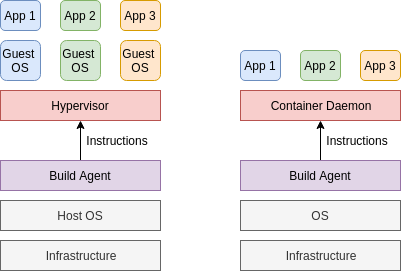
\includegraphics[width=.7\textwidth]{figures/drawio/build-agent.png}
    \caption{\textit{Overview of build agents and their relation to virtual infrastructure.}}
    \label{fig:build-agents} 
\end{figure} 


\subsection{Security Tools} \label{subsec:security}
There are many automated security tools available that can analyze static code or programs during execution to find known vulnerabilities or point to functions/behavior that could be indicative of an underlying problem. Some DAST-tools (Dynamic Application Security Testing) are specialized in exposing web application related vulnerabilities by fuzzing APIs or performing automated SQL (Structured Query Language) injection attacks while SAST-tools (Static Application Security Testing) might look at insecure configuration options or imports of vulnerable libraries.\cite{owasp-tools,owasp-sast} Some CI/CD solutions offer "\textit{Security as a Service}"-support and use similar SAST/DAST tools under the hood.\cite{gitlab-sast,gitlab-dast} There are tools available that manage and analyze code dependencies and any binaries or other artifacts that might get produced as well.\cite{jfrog}

The following list of tools is by no means comprehensive, but are merely some that are either widely used, open-source or have good Python integrations. Some of these will also be discussed during the implementation phase described in Chapter \ref{chapter:implementation}.

\pagebreak

\subsubsection{Clair}
Clair is a container analysis tool that looks for known vulnerabilities in dependencies and libraries used in container recipes.\cite{clair,clair-scanner} It looks at the various layers that comprise a container and checks against multiple open databases and bug trackers to see if one of these is included in the container. Some of these databases include NIST NVD (National Vulnerability Database), Alpine SecDB, RedHat Security Data and Ubuntu CVE tracker (Common Vulnerabilities and Exposures).\cite{clair}

\subsubsection{Bandit}
Bandit is a linter, SAST and code analysis tool that finds common security issues in Python code.\cite{bandit} It supports generating reports in JSON (JavaScript Object Notation), HTML (Hypertext Markup Language) and XML among others. Its modules look for weak ciphers used, hardcoded passwords, insecure deserialization using \textit{pickle} and usage of the \textit{eval} command to just name a few. Although one can also write their own modules for it. Analyzing your code can be done fairly easily through issuing a simple command like in Figure \ref{fig:bandit-command}.

\begin{figure}[H]
\centering
\begin{lstlisting}[frame=single, basicstyle=\small, linewidth=\textwidth]
bandit -r path/to/your/python/code -f xml -o bandit-results.xml 
\end{lstlisting}
\caption{\textit{Example Bandit analysis command.}}
\label{fig:bandit-command}
\end{figure}
Many CI/CD servers allow for some sort of artifact uploading, either natively or through the use of plugins. If there is support for the specific format of the test results these can sometimes be nicely parsed and visualized in the CI/CD server, but reports can alternatively be uploaded to the server's artifact repository for later manual analysis. Figure \ref{fig:bandit-output} is part of the \textit{Bandit} report that was created when the previous command was run on the example application that was developed during the analysis phase described in Chapter \ref{chapter:analysis}.

\begin{figure}[H]
\centering
\begin{lstlisting}[frame=single, basicstyle=\small, linewidth=\textwidth]
Test results:b201_flask_debug_true.html
>> Issue: [B201:flask_debug_true] A Flask app appears to be run 
          with debug=True, which exposes the Werkzeug debugger 
          and allows the execution of arbitrary code.
   Severity: High   Confidence: Medium
   Location: example/app.py:55
   More Info: https://bandit.readthedocs.io/en/latest/plugins/
              b201_flask_debug_true.html
54	if __name__ == '__main__':
55	    app.run(host='0.0.0.0', port=80, debug=True)
\end{lstlisting}
\caption{\textit{Bandit analysis result output.}}
\label{fig:bandit-output}
\end{figure}

\subsubsection{SonarQube}
SonarQube can find code smells, bugs and security vulnerabilities in code.\cite{sonarqube} It provides a CLI (Command Line Interface) scanning tool and databases with known vulnerabilities to do so. It can also nicely visualize \textit{Pytest}, \textit{Coverage}, \textit{Pylint} and \textit{bandit} reports if they are formatted in either JUnitXML or JSON notation. Some of these and their alternatives will also be discussed in section \ref{subsec:other}. It is an interesting tool to help combat regression and security issues by generating, combining and visualizing code quality metrics. 


\subsubsection{Black Duck}
Black Duck is a security tool that can perform binary analysis (e.g. executables and archives), dependency analysis and file system scans to detect vulnerabilities. It integrates with large deployment frameworks like RedHat OpenShift to perform automated scans on container clusters. It can also identify potential license conflicts that arise due to imported code.\cite{black-duck}

\subsubsection{OpenSCAP}
SCAP (Security Content Automation Protocol) is a framework of open standards maintained by NIST and OpenSCAP is a set of tools used to implement this standard which allows for automated configuration and vulnerability scans of computer systems.\cite{mitre-oval} It can do this through the use of XCCDF (Extensible Configuration Checklist Description Format) and OVAL (Open Vulnerability and Assessment Language) files which consist of XML-based descriptions of machine state and system information and link these to security issues.\cite{openscap,openscap-manual} When for example a new vulnerability is discovered, one can write such a file describing the conditions in which the vulnerability appears. Tools like the by OpenSCAP provided \textit{oscap,} are able to scan through these files and discover if any of these described conditions occur on the system it is running on. Repositories for these files are published by companies and projects like Cisco, RedHat, Debian and NIST (National Institute of Standards and Technology).\cite{oval-repo} There are also enterprise level integrations in the form of RedHat container vulnerability management (Atomic Scan) and system management through RedHat Satellite profiles.\cite{openscap-tools}

\pagebreak

\subsubsection{OWASP ZAP}
The ZAP project is an open-source security testing tool supported by OWASP (Open Web Application Security Project). It can be set-up in between a browser and a web application as a proxy and analyzes traffic during interactions to detect common vulnerabilities like SQL-injections. It supports both passive scans as well as active scans of your web application using a wide variety of extensions.\cite{owasp-zap,owasp-zap-ext} See also section \ref{subsec:other} for information on Selenium Web browser, in combination of which this could be used to automate security tests.

\subsection{Other} \label{subsec:other}
\subsubsection{Functional Testing}
A framework that is often used for automated functional testing of web applications and their GUIs is \textit{Selenium WebDriver} which can run tests against many popular browsers like Chrome, Firefox, Edge and Safari.\cite{selenium} It does this by obfuscating away any actual HTML interactions from the tests through what's called a PageObject pattern.\cite{fowler-page} It has good integrations with Python as well.\cite{selenium-python}

\subsubsection{Code Coverage}
Writing and passing tests should raise the confidence one has in the proper functionality of the code under test. But how does one know how well these tests reflect the code's functionality? Code coverage refers to metrics that reflect how much code has been executed during the running of tests. They can be a measure of how well tests are written since a higher coverage percentage reduces the chance of any bugs remaining in the code. They generally come in a few forms: \textit{branch coverage}, \textit{statement coverage}, \textit{function coverage} and \textit{condition coverage}. High code coverage percentages don't guarantee high quality of code.\cite{cov-misuse} And 100\% statement coverage does not guarantee 100\% branch coverage, as can be seen in the example in Figure \ref{fig:codecoverage} where, given test situation \textit{a='true'} and \textit{b='true'}, there is 100\% statement coverage but two-thirds of the branches are not covered.

\begin{figure}[!htb]
    %\begin{minipage}{0.5\textwidth}
    \begin{subfigure}[b]{0.5\textwidth}
    \begin{lstlisting}[frame=single, basicstyle=\small, linewidth=.9\textwidth]
# given a=true and b=true
if(a){
    if(b){
        bool example = true;
    }
}
    \end{lstlisting}
    \end{subfigure}
    %\end{minipage}%
    %\begin{minipage}{0.5\textwidth}
    \begin{subfigure}[b]{0.5\textwidth}
    \centering
    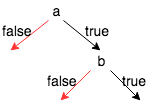
\includegraphics[width=.75\textwidth]{figures/branch-statement.png}
    \end{subfigure}
    %\end{minipage}
    \caption{\vspace{-3mm}\textit{Branch coverage vs. Statement coverage.}\cite{stack-cov}}
    \label{fig:codecoverage}
\end{figure} 

There are tools that can create these reports for most popular languages and Python is no exception to this. \textit{Coverage} and \textit{pytest-cov}\cite{pytest-cov} both support generating coverage reports which can in turn be submitted to tools like \textit{codecov} or \textit{opencov} and the earlier mentioned \textit{SonarQube} for visualizations.\cite{codecov} This is done by monitoring the code during test execution.

\subsubsection{Linters \& Code Analysis}
Coding standards and language specific styling rules are subjective, but adhering to these can increase overall code quality by creating readable, clean code. Linters can help enforce these rules as well as detect errors, dangerous code patterns as well as help with refactoring of your code at the same time. PEP8 is the style guide for Python.\cite{pep8} Some popular linters for Python are Flake8 and Pylint.\cite{pylint} Other more security oriented code analysis tools are talked about in Section \ref{subsec:security}.

\subsubsection{Badges}
Communicating metrics and overall health of a project can be important for open source projects. It can increase confidence in a project's functionality for users who might need to decide between using similar tools. Badges are images that communicate these metrics and general information in a human-friendly way. They are generally incorporated on repository READMEs or other communication pages and there are a wide variety of them.\cite{shields} Many CI/CD servers have some way to generate build-status badges.

% TODO: Add more information on VPN technology?
%\section{Tunneling Technologies}
%OpenVPN / StrongSwan as opposed to WireGuard..  (\url{https://www.wireguard.com/papers/wireguard.pdf})
%\url{https://en.wikipedia.org/wiki/Tunneling_protocol}
%Relevant because the main use-case of Certidude is certificate based VPN tunneling.




\chapter{Analysis}\label{chapter:analysis}
This chapter will describe multiple CI/CD server implementations and contains an analysis of their relevance to Certidude and adherence to the requirements that are defined in the first section of this chapter. The chapter ends with a short review, discussion and conclusion.

The analysis of the tools also required a hands-on approach to determine which would be best suited. A dummy application was developed, based on Python and the Flask web framework. Two almost-identical test suites were created to test this application: one based on Flask fixtures, the other using Docker and raw HTTP (Hyper Text Transfer Protocol) requests. It was pushed to two separate version control systems: a public Github repository\cite{korving-example} and a privately hosted Gitlab repository. This was done since some CI/CD solutions are public cloud based, while others are privately hosted. The public repository contains the created pipeline definition files for all solutions  which can additionally be found in Appendices \hyperref[chapter:appendix-travis]{1}, \hyperref[chapter:appendix-jenkins]{2}, \hyperref[chapter:appendix-gitlab]{3}, \hyperref[chapter:appendix-tc]{4} and \hyperref[chapter:appendix-circleci]{5}.

Unfortunately there are too many CI/CD solutions available to make testing them all a feasible task. A selection was made based on variation in properties like popularity, applicability, licensing, community vs. proprietary support and whether the service is hosted in the cloud or on premises. This selection should reflect the CI/CD landscape in general, but left out popular solutions like: Bitrise (for mobile applications), GoCD, Bamboo/Bitbucket Pipelines, Codeship, Azure DevOps (formerly known as VSTS) and Zuul-CI.\cite{bitrise, gocd, vsts, bamboo, zuul}

\pagebreak

\section{Solution Requirements} \label{analysis:requirements}
Table \ref{table_cicd_requirements} contains the requirements needed from the tools under test. Each requirement is numbered and has a weighted grading ranging from "\textit{High}" (essential) to "\textit{Medium}" (recommend) to "\textit{Low}" (desirable).
After the table these requirements are discussed in more detail.

\begin{longtable}{|p{0,5cm}|p{10cm}|p{3cm}|}
	\caption{\it{CI/CD solution requirements}}
	\label{table_cicd_requirements}\\ \hline
	\textbf{Nr} &  \textbf{Requirement} & \textbf{Weight}  \\
	\hline
	\endfirsthead
	\multicolumn{3}{l}%
	{\tablename\ \thetable\ -- \textit{Continues...}} \\
	\hline
	\textbf{Nr} &  \textbf{Requirement} & \textbf{Importance}  \\
	\hline
	\endhead
	\hline \multicolumn{3}{l}{\textit{Continues...}} \\
	\endfoot
	\hline
	\endlastfoot
1 & Affordability & High\\ \hline
2 & Variety of Supported Up-to-Date Build Environments& High\\ \hline
3 & Integrations available (e.g. Git/Docker)& High\\ \hline
4 & Maintainability& High\\ \hline
5 & Learning Curve& High \\ \hline
6 & Good and Intuitive UX& Medium\\ \hline
7 & Configuration in VCS& Medium\\ \hline
8 & Extensive and Up-to-Date Documentation & Medium\\ \hline
9 & Scalability and Performance & Medium\\ \hline
10 & Public vs. Private& Medium\\ \hline
11 & Open-Source & Low\\ \hline
12 & Dashboards and Metric Visualizations & Low\\ \hline
\end{longtable}

\textbf{High}\\
\textit{Requirement 1} covers pricing of the chosen CI/CD solution, which should be either free or at least affordable, especially since Certidude is an open-source project. \textit{Requirement 2} covers the CI/CD solution's ability to run and test code in up-to-date versions of a wide variety of operating systems. \textit{Requirement 3} touches on the fact that the tool needs to be able to integrate well with 3rd party solutions like version control systems, code coverage visualization tools and virtualization technologies. \textit{Requirement 4} deals with the amount of post-installation effort to keep-up a healthy state of the solution. \textit{Requirement 5} covers the fact that it shouldn't be too difficult to learn how to install, maintain and use the tool or essential components like pipeline definition languages which have to be used.

\pagebreak

\textbf{Medium}\\
\textit{Requirement 6} covers that important information and features need to be easily findable as well as having clear pipeline status visualizations. It would be a good thing if the configuration file which contains the pipeline definition(s) is part of the same version control system as the code that is being tested. This is covered by \textit{Requirement 7}. \textit{Requirement 8} deals with the amount and detail of published documentation as well as publicly available ticket systems which can be essential while trying to debug technical problems. This might also be an indication of overall community support and health of the project. \textit{Requirement 9} describes that the tool needs to be fast and be able to deal with multiple parallel tasks. If resources are insufficient it should be scalable to fit demand. (\textit{Requirement 10}) covers support for both public as well as private repositories, in case Certidude will have a commercial version in the future.

\textbf{Low}\\
Less important, but still desirable traits of the CI/CD solutions would be that the tool itself is an open-source project (\textit{Requirement 11}) and having performance metrics visualizations (\textit{Requirement 12}). This last part is especially relevant for self-hosted solutions where one wants to keep an eye out for resource consumption and increase in execution times.


\section{Overview of Tested Solutions}
%https://instabug.com/blog/continuous-integration-tools/
%Some points of comparison:
%Features (without plugins) / supported Platforms
%On Demand Builds	/ Parameterized Builds / Handling Secrets / Sandboxed Builds
%Configs with Repository	"Automatic pipeline creation for organizations"
%Metrics	/ Dashboard / Reusable Tasks Jobs / Status Matrix 
%/ Good and Friendly UX / Github PR Support / Public Builds
%
This section describes the selected CI/CD solutions as well as how they were installed, configured and tested. If an interesting or distinguishing feature was found, it will be discussed and/or shown how it was implemented. The main test device used was a private server running \textit{Ubuntu 16.04.5 LTS (GNU/Linux 4.4.0-141-generic x86\_64)}. The pipeline definition files for on premise solutions were initially hosted on a private Gogs instance, but were moved to Gitlab once it was installed to test its embedded CI/CD solution. Additionally on premise solutions require build agents to perform defined tasks. For sake of testing purposes these were simply setup on the host machine itself.

\pagebreak

\subsection{Jenkins}
\begin{wrapfigure}{r}{.3\textwidth}
    \vspace{-50pt}
    
\includegraphics[width=.3\textwidth]{figures/brand/jenkins.jpeg}  
    \vspace{-30pt}
\end{wrapfigure}
\textbf{Name}: Jenkins (associated with: \textit{Hudson} , \textit{Cloudbees})\\
\textbf{Website}: \url{http://jenkins.io}\\
\textbf{Documentation}: \url{https://jenkins.io/doc/}\\
\textbf{Hosting type}: Self-Hosted

Jenkins is a Java-based, on premise, open source CI/CD server published under a MIT-license and originally developed by Sun Microsystems. Originally it was known as Hudson, but this project was forked after Oracle's acquisition of Sun and the entire development community associated with the project moved over to Jenkins instead. It has a commercial version called Cloudbees. Their developers contribute to the main Jenkins codebase as well as have added some custom plugins geared towards enterprise environments.\cite{cloudbees} 

Jenkins server can be easily installed through \textit{Debian} packages, RedHat \textit{RPM} packages (Red Hat Package Manager), FreeBSD's \textit{pkg} package manager or a Windows installer. OpenJDK was installed instead, a Jenkins \textit{WAR} (Web application ARchive) was downloaded and executed which started an embedded web server and the application running on top of it.\footnote{Not recommended for a permanent installation, but has no limitations that would hinder a test run.} Jenkins slaves (build agents) can be setup over ssh or registered through downloading an application through the GUI (Graphical User Interface) of the web page on the target machine.
\begin{figure}[H]
\centering
\begin{lstlisting}[frame=single, basicstyle=\small, linewidth=\textwidth]
java -jar jenkins.war --httpPort=8081
\end{lstlisting}
\caption{\textit{Starting the Jenkins web server.}}
\label{fig:jenkins-start}
\end{figure}

A special text file with the name "\textit{Jenkinsfile}" contains the pipeline definition and can be included in the repository you are creating the pipeline for. Jenkins allows for two syntax flavors: scripted and declarative.\cite{jenkins-dsl, jenkins-declarative} The former being a Groovy-based DSL, which gives access to most of Groovy's inbuilt functionality for more advanced use-cases.
This file was created for the test application with its declarative syntax and can be seen in Appendix \hyperref[chapter:appendix-travis]{1}.

\pagebreak

No build agents were tagged to run specific tasks so mostly the main master build agent was used. Jenkins exposes an API through which one can trigger builds or retrieve status updates. This was used to setup a webhook between VCS and Jenkins, as well as have a nice looking build-status badge on the project's README. Jenkins can do a lot by itself, but one of it's main strengths is the amount of community support and the number of plugins available to extend its functionality. One of the main ones that was installed for this test was something called \textit{BlueOcean}. It both updated the slightly outdated GUI with a slick new look and added an intuitive point-and-click pipeline editor.


\subsection{Gitlab}
\begin{wrapfigure}{r}{.25\textwidth}
    \vspace{-50pt}
    
\includegraphics[width=.25\textwidth]{figures/brand/gitlab-ci-cd-logo_2x.png}  
    \vspace{-30pt}
\end{wrapfigure}
\textbf{Name}: Gitlab CI/CD \\
\textbf{Website}: \url{https://about.gitlab.com/}\\
\textbf{Documentation}: \url{https://docs.gitlab.com/ee/ci/}\\
\textbf{Hosting type}: Self-Hosted and Cloud

Gitlab is an open-core git repository management tool with an embedded CI/CD server and registries to manage docker images and artifacts written in Ruby and Go. One can make use of the cloud hosted version on \url{gitlab.com} that comes with build agents (\textit{runner} in their vernacular) or a self-hosted version where one can install build agents on Windows, Linux and FreeBSD machines alike. Premium features are offered as a service like SAST/DAST/Container and dependency scanning capabilities but are offered for free for open source projects if going for the cloud.

The self-hosted server was installed alongside a build agent and the docker registry was configured so as to push built Docker images. Enterprise Edition (EE) was installed but only Community Edition (CE) functionality is used, which is published under an MIT license. Appendix \hyperref[chapter:appendix-gitlab]{3} shows the pipeline definition file for the test application. It is a special text file with the name "\textit{.gitlab-ci.yml}" and is written in a declarative YAML syntax. This makes the language less powerful than for example the Groovy-based engine Jenkins can use but is also easier to learn while being powerful enough to scale and implement most use-cases. It incorporates programming concepts as variables, conditional execution and inheritance.

\pagebreak

It has inbuilt badge creation capabilities and comes with multiple ways to report on code coverage by parsing out standard output coming from the build agent. Natively one would add a regular expression to the project's configuration page, but this can be added as a job definition as well, like the following block shows.
\begin{figure}[H]
\centering
\begin{lstlisting}[frame=single, basicstyle=\small, linewidth=\textwidth]
test-job:
  script: pytest --cov=example/ tests/
  coverage: '^TOTAL\s+\d+\s+\d+\s+\d+\s+\d+\s+(\d+\%)$'
\end{lstlisting}
\caption{\textit{Gitlab regex-based parser for Pytest results.}}
\label{fig:test-regex}
\end{figure}

Secrets can be defined for the project and accessed through variables in the pipeline definition. This can be done through global variables or temporary ones defined when manually running the build. Figure \ref{fig:gitlab-vars} shows these variables being used in the created pipeline for the test application when it is interacting with the configured Docker registry. See Appendix \hyperref[chapter:appendix-gitlab]{3} for the full file.
\begin{figure}[H]
\centering
\begin{lstlisting}[frame=single, basicstyle=\small, linewidth=\textwidth]
... Building and pushing the container
    - docker login -u $REG_UNAME -p $REG_PASSWORD $REG_TARGET 
    - docker build -t $TEST_NAME .
    - docker push $TEST_NAME
    
... Pulling and running the container
    - docker login -u $REG_UNAME -p $REG_PASSWORD $REG_TARGET
    - docker pull $TEST_NAME
    - docker run -dt -p 8282:80 -v $PWD:/tmp/ --name \ 
                               gitlabCICDContainer $TEST_NAME
\end{lstlisting}
\caption{\textit{Gitlab variables and Docker registry interaction.}}
\label{fig:gitlab-vars}
\end{figure}

Gitlab CI is definitely the easy to learn, all-in-one solution where developers and administrators get more for less. No need for an additional repository management tool, wiki-solution for documentation, separate docker registry instance and CI/CD server. This is great for at least small to medium sized projects where this might save valuable and scarce resources.

\pagebreak

\subsection{TeamCity}
\begin{wrapfigure}{r}{.25\textwidth}
    \vspace{-50pt}
    
\includegraphics[width=.25\textwidth]{figures/brand/teamcity.png}  
    \vspace{-30pt}
\end{wrapfigure}
\textbf{Name}: TeamCity by Jetbrains\\
\textbf{Website}: \url{https://www.jetbrains.com/teamcity/}\\
\textbf{Documentation}: \url{https://confluence.jetbrains.com/display/TCD18/TeamCity+Documentation}\\
\textbf{Hosting type}: Self-Hosted

TeamCity is a Java-based, commercial CI/CD server created by JetBrains which has a limited freemium version for closed source projects but free licenses can be applied for if the project is open source. 

OpenJDK was installed, after which the TeamCity tarball was downloaded and unpacked. It provides a script through which to run and stop the server. It adds a build agent on the same machine as the server by default which was used to run the test builds. See also Appendix \hyperref[chapter:appendix-tc]{4} for the pipeline created for the test application which for TeamCity goes by the special filename "\textit{settings.kts}".

TeamCity offers agent pools, test analysis and history on a per-test basis as well as interesting native integration options like Sysinternal's psexec, issue trackers and S3 storage for build artifacts. It offers metric visualizations like resource consumption and build times. It can integrate well with popular IDEs and version control systems which is necessary because the Kotlin-based pipeline definitions are mainly created using the GUI-based editor and this allows the instance to also write any updates to the pipeline to the project's repository.

TeamCity feels like a mature tool with significant native support for .NET and Java applications by integrating with tools like Ant, Gradle, Maven and MSBuild.
\pagebreak

\subsection{Travis CI}
\begin{wrapfigure}{r}{.25\textwidth}
    \vspace{-50pt}
    
\includegraphics[width=.25\textwidth]{figures/brand/TravisCI-Mascot-1.png} 
    \vspace{-30pt}
\end{wrapfigure}
\textbf{Name}: Travis CI\\
\textbf{Website}: \url{https://travis-ci.org}\\
\textbf{Documentation}: \url{https://docs.travis-ci.com/}\\
\textbf{Hosting type}: Cloud

Travis CI is a cloud based CI/CD platform written in Ruby. It has a free version for open source projects hosted on Github and an enterprise, paid version that can be deployed on premise. The latter being considered out-of-scope for this analysis. It integrates for free with tools like \textit{codecov.io} for coverage report visualizations and \textit{coverty/pyup} for static analysis scans when the project is open source.\cite{pyup}

Since Travis CI is cloud based, one does not have control over build agents. Instead build environments are automatically provisioned for the user and are available in limited amounts and variety. As of this writing they support the following VMs: Windows Server 1803, macOS 10.10-14 and Ubuntu 12.04 / 14.04 and since recently also 16.04. 

Connecting Travis CI to Github was an almost trivial task where one authorizes Travis CI as an OAuth application in Github and sets up webhooks back to Travis CI for those projects you choose to connect. A "\textit{.travis.yml}" file with a YAML based declarative pipeline was created and included in the repository which Travis CI automatically looks for to execute. The full pipeline for the test application can be found in Appendix \hyperref[chapter:appendix-travis]{1}. 

Codecov was similarly integrated with Github, an API token was generated and included in the Travis CI project as an environmental variable (CODECOV\_TOKEN) for any triggered build. Figure \ref{fig:travis-codecov} shows part of the developed pipeline where a coverage report is generated and transparently uploaded to Codecov's web page under condition that all tests passed (i.e. return code of pytest command was 0).
\begin{figure}[H]
\centering
\begin{lstlisting}[frame=single, basicstyle=\small, linewidth=\textwidth]
- stage: test
  name: "Running functional tests with fixtures"
  script:
    ...
    - pytest --cov-report term --cov-branch \
                               --cov=example/ tests2
  after_success:
    - codecov
\end{lstlisting}
\caption{\textit{Travis CI and Codecov pipeline integration.}}
\label{fig:travis-codecov}
\end{figure}

Conditional execution of stages are possible as well. Here the \textit{deploy} stage and its code is only executed when the previous build steps passed and the current branch is master.
\begin{figure}[H]
\centering
\begin{lstlisting}[frame=single, basicstyle=\small, linewidth=\textwidth]
stages:
  - build-run-test
  - test
  - name: deploy
    if: branch = master
\end{lstlisting}
\caption{\textit{Travis CI and conditional pipeline execution.}}
\label{fig:travis-conditional}
\end{figure}

\subsection{CircleCI}
\begin{wrapfigure}{r}{.25\textwidth}
    \vspace{-50pt}
    
\includegraphics[width=.25\textwidth]{figures/brand/circleci2.png}  
    \vspace{-30pt}
\end{wrapfigure}
\textbf{Name}: CircleCI\\
\textbf{Website}: \url{https://circleci.com}\\
\textbf{Documentation}: \url{https://circleci.com/docs/}\\
\textbf{Hosting type}: Self-Hosted and Cloud

CircleCI is an enterprise CI/CD solution that can be either utilized in the cloud or through an on premise installation. The latter will be considered out-of-scope for this analysis. It offers 4 free hosted containers without build-time limits for open source projects although some features are still for paid users only. There is support the following execution environments: Docker, Linux VM or macOS. The pipeline file created for the test application is written in YAML and placed in the directory / path "\textit{.circleci/config.yml}" where CircleCI looks by default.

One can use any publicly hosted Docker image, build one in the pipeline itself or use images provided as a service by CircleCI itself which saves time building it. They also offer something called "\textit{Docker Layer Caching}" as a paid service. This allows one to "carry over" stored layers of built Docker images to next tasks which make use of the same images and speeds up the execution of the pipeline. While ignored using it with the free, open source license it is used in the example pipeline file found in Appendix \hyperref[chapter:appendix-circleci]{5} as well.

CircleCI makes use of something called "Orbs" which allow for importing and abstracting away large blocks of functionality in the pipeline. One feature that made working with CircleCI pleasant was that a code base can be pushed through a pipeline job submitted through an API request, overriding the default file located at "\textit{.circleci/config.yml}". 
\pagebreak

This is useful to test new versions of the pipeline without having to create a commit in your VCS repository and is an alternative to using a dedicated branch to do such experiments. Figure \ref{fig:circle-api} shows such a request.

\textit{CIRCLE\_TOKEN} is a generated API token for CircleCI set as an environmental variable on the development machine, \textit{build\_parameters} refers to the named job that needs to be run and \textit{revision} is the commit hash of the code under test.

\begin{figure}[H]
\centering
\begin{lstlisting}[frame=single, basicstyle=\small, linewidth=\textwidth]
curl --user ${CIRCLE_TOKEN}: \
     --form config=@config.yml \
     --form notify=false \
     --form revision=f8e527e1c2b79f6c0c68761018dc3e3e4b08b0c0 \
     --form build_parameters[CIRCLE_JOB]=build-fixtures \
     --request POST "https://circleci.com/api/v1.1/project/
               github/Korving-F/thesis-cicd-examples/tree/master"
\end{lstlisting}
\caption{\vspace{-3mm}\textit{CircleCI API call to trigger a build.}}
\label{fig:circle-api}
\end{figure}

\section{Comparison of Tested Solutions}
Table \ref{table_cicd_comparison} shows a comparison between the five tools under test and the requirements defined in Table \ref{table_cicd_requirements}. The evaluations are based on the functionality and license that came with the tools as tested. This means full functionality for Jenkins and Travis, limited functionality for Gitlab and limited amount of build agents/configurations for TeamCity and CircleCI. Some scores are based on the author's subjective opinion that formed while working with the tools and should not be interpreted as hard fact. Other low scores were given because of the tool's lack of applicability to Certidude. Comments will be given to justify some of the outliers. The scores are relative to the other tools on the same requirement and are between '++' good, '+' average and '-' bad, difficult to achieve or missing.

Travis CI got a low score for the "\textit{Supported build environments}" requirement because of delays in up-to-date Linux distribution VM provisioning (support for Ubuntu 16.04 was released months before 14.04 reached end of life). 

Both cloud based solutions are scored as being very maintainable since one doesn't have to be concerned with any hardware or installation of agents. Gitlab got additional points compared to the other on premise tools on this requirement because it eliminates other services that could be running on premise, like a hosted git repository.

\pagebreak

The learning curve for tools like Jenkins and TeamCity is deemed steeper than the other tools which is partly due to the pipeline definition languages they use. It is the author's feeling that this in turn could make them more relevant in more complex setups where there are many developers across dozens of projects with dozens of branches, each having their own pipelines defined. This is why Jenkins got more points in the scalability requirement. TeamCity's license puts limits on the amount of available build agents, so while there's potential it's less relevant to the version/license under test. 


\begin{longtable}{|p{4.5cm}|p{1.8cm}|p{1.8cm}|p{1.8cm}|p{1.8cm}|p{1.8cm}|}
	\caption{\it{CI/CD server comparison}}
	\label{table_cicd_comparison}\\ \hline
	\textbf{Feature / Requirement} &  \textbf{GitlabCI 11.9.2-ee 11.9.8-ee} & \textbf{TravisCI Cloud} & \textbf{CircleCI Cloud} & \textbf{Jenkins v2.150.3} & \textbf{TeamCity 2018.2.2}  \\	\hline
	\endfirsthead
	\multicolumn{6}{l}%
	{\tablename\ \thetable\ -- \textit{Continues...}} \\
	\hline
	\textbf{Feature / Requirement} &  \textbf{GitlabCI 11.9.2-ee} & \textbf{TravisCI} & \textbf{CircleCI} & \textbf{Jenkins v2.150.3} & \textbf{TeamCity 2018.2.2}  \\
	\hline
	\endhead
	\hline \multicolumn{6}{l}{\textit{Continues...}} \\
	\endfoot
	\hline
	\endlastfoot
	%High
	\textbf{HIGH}   \\ \hline
	Affordability 			                                & ++ & +\footnotemark & +\footnotemark[\value{footnote}] & ++ & + \footnotetext{Pricing heavily dependent on the project remaining open source}\\ \hline 
	Supported Build Environments 	                    	& ++ & - & + & ++ & +\\ \hline
	Integrations available                                  & + & + & + & ++ & +\\ \hline
	Maintainability                                         & + & ++ & ++ & - & -\\ \hline
	Learning Curve                                          & ++ & ++ & ++ & - & -\\ \hline
	%Medium
	\textbf{MEDIUM} 	  \\ \hline
	Good and Intuitive UX (User Experience)                 & ++ & ++ & ++ & - & - \\ \hline
	Configuration in VCS	                                & + & + & + & + & + \\ \hline 
	Documentation Quality                                   & + & + & + & + & + \\ \hline
	Scalability and Performance                            	& + & -\footnotemark & -\footnotemark[\value{footnote}] & ++ & + \footnotetext{Performance heavily dependent on availability of resources. Resource queues and outages are know to have occurred for both solutions}\\ \hline
    Public vs. Private		                                & ++ & - & - & ++ & ++ \\ \hline
	\textbf{LOW} 	  \\ \hline
	Open-Source			                                	& + & - & - & ++ & -\\ \hline
	Dashboards and Metric Visualizations               		& + & + & + & + & +\\ \hline
\end{longtable}
\pagebreak

\section{Considerations and Conclusion}
As one could see in Chapter \ref{chapter:concepts} there are many interesting and helpful components a CI/CD pipeline can consist of. Setting up and maintaining all these tools could get very complicated, costly and time consuming very quickly which might not seem worth the effort for a small team at first.\cite{cicd-review} Other barriers like resistance to workflow and process changes are also sometimes mentioned.\cite{comparison-cicd} It is however automating good practices which otherwise would have to be performed manually and which catch problems at an earlier stage as well. This is where an implemented CI/CD server starts to return on its initial investment quickly.\cite{comparison-cicd}

Most of the tools could fulfill most of the basic needs of a small project, but when used for more advanced use cases or with larger projects suitability becomes dependent on context. \textit{What languages are being used? What resources are available to the project? Is the project open source? Is there a need of enterprise level support?} This is an evaluation that should be done on a per project basis.

While according to the author Jenkins was the most capable it was also less easy to learn than its alternative which was not deemed a worthwhile trade off for a relatively small project like Certidude. For Certidude the switch from TravisCI to GitlabCI will be made. It is open source, powerful, versatile and fairly easy to learn. It has no very obvious downsides while performing good on most points. It was also deemed a good fit by the main developer and supervisor of this thesis \supervisor. Implementation will be discussed in Chapter \ref{chapter:implementation}.

\chapter{Implementation}\label{chapter:implementation}
This chapter discusses some of the functionality that was implemented for Certidude in Gitlab, the chosen CI/CD solution. Preparatory work included the needed migration from Certidude's publicly hosted git repository on Github to the (so far) private Gitlab instance that was setup during the analysis phase described in Chapter \ref{chapter:analysis}. 

Section \ref{sec:pylint-pytest-bandit-sonarqube} describes the setup of an initial pipeline for Certidude where code quality tools are integrated to analyze Certidude's code base. See Chapter \ref{chapter:concepts} for more details on these tools. Section \ref{vbox-cert} describes how new build environments can be provisioned using the Gitlab VirtualBox runner. Section \ref{openwrt} describes an implemented step in the pipeline to compile OpenWrt images. This chapter concludes with section \ref{future-work}, where a list was compiled of features and tasks that would expand and improve upon this work.

Appendices \hyperref[chapter:appendix-certidude-pipeline]{6}, \hyperref[chapter:appendix-sonar]{7}, \hyperref[chapter:appendix-vbox]{8} and \hyperref[chapter:appendix-openwrt]{9} contain produced configuration files, pipeline definition files and used instructions to produce a VirtualBox based build agent which can launch a VM and integrate with Gitlab CI.

\section{Pylint, Pytest, Bandit and SonarQube} \label{sec:pylint-pytest-bandit-sonarqube}
A basic pipeline was created with \textit{build, test and scan} stages for Certidude and the associated YAML file was included into the repository so as to be able to trigger it. See Appendix \hyperref[chapter:appendix-certidude-pipeline]{6} for the full declaration of this pipeline. Its \textit{build} phase contains one task: "\textit{sonar\_docker}". It starts a docker image containing SonarQube by first pulling it from the docker repository which is integrated into Gitlab and then issuing the command to initiate its main process. This sets up the web service that will later take in and visualize test and scan reports. 

The inbuilt docker registry of Gitlab is hosted by default through port 5001. The following commands show how the docker image provided by SonarQube was pulled from their public repository, tagged and pushed to Gitlab's private one. This was mainly done to help speed up the build process.

\pagebreak

\begin{figure}[H]
\centering
\begin{lstlisting}[frame=single, basicstyle=\small, linewidth=\textwidth]
user@host:~# docker login -u <username> -p <password> \\ 
                                        <ip/host>:5001
user@host:~# docker pull sonarqube
user@host:~# docker tag sonarqube:latest \\
                    <ip/host>:5001/certidude/certidude:sonarqube
user@host:~# docker push <ip>:5001/certidude/certidude:sonarqube
\end{lstlisting}
\caption{\textit{Pushing a SonarQube image to the Docker registery in Gitlab.}}
\label{fig:gitlab-sonar-docker}
\end{figure}

The \textit{test} stage contains three tasks: "\textit{Pylint, Pytest and Bandit}". These three parallel tasks each produce report artifacts which are uploaded to Gitlab. They indicate which tests passed or failed, which lines of code were covered by those tests, conformity to coding standards and possible security issues encountered. These reports are produced in a structured format (e.g. JSON / XML) and which are later consumed by SonarQube. The "dependencies" section of a task in Gitlab's YAML syntax is needed to indicate what earlier produced artifacts will be downloaded into the working directory where the current task is being executed.

In the final \textit{scan} stage we can see one task "\textit{sonar\_scan}" which takes in all previously generated reports. It also installs SonarQube's active scanner utility and scans Certidude's code based on a profile of defined rules hosted on the previously started SonarQube instance. See Figure \ref{fig:sonarqube-profiles} for how the default Python profile was extended to include more rules. The utility needs a configuration file to interact with the main server which was included in Appendix \hyperref[chapter:appendix-sonar]{7}. After the scan is complete the utility uploads its results and all the previously generated reports to the main SonarQube server for visualization and analysis. Figure \ref{fig:sonarqube-result} shows part of Certidude's results visualized in SonarQube. Here all previously gathered reports and information is condensed into one place. The following points describe parts of the image.

\begin{enumerate}
    \item Name of the project and file currently under review. The project was named \textit{Certidude} and \textit{cli.py} is currently being analyzed.
    \item A vulnerability rule was triggered and this indicates the offending line. A variable command is executed in a subshell which could indicate a possibility of command injection if the variable is manipulable.
    \item Source of this triggered rule, in this case the report generated by \textit{Bandit}. It also shows the inbuilt ticketing system and classification of the triggered rule.
    \item Shows the date and commit hash identifying when this piece of the code was contributed.
    \item Red and green annotations placed next to each line are based on the provided code coverage reports and indicate whether that line was executed during the tests. 
\end{enumerate}

\begin{figure}[!htb]
    \centering
    \begin{minipage}{.5\textwidth}
        \centering
        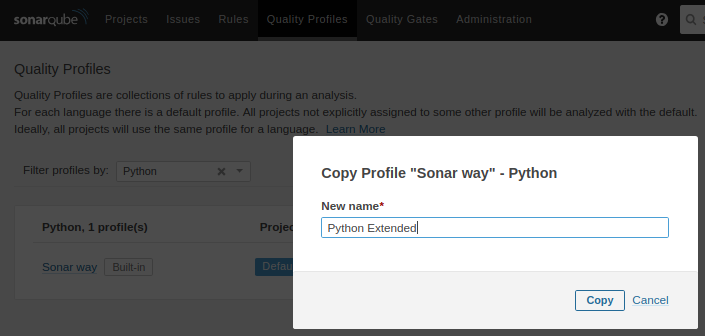
\includegraphics[width=.95\linewidth]{figures/screenshots/sonar-profile.png}
    \end{minipage}%
    \begin{minipage}{0.5\textwidth}
        \centering
        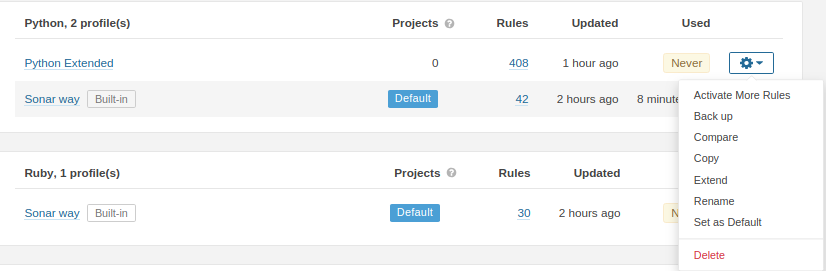
\includegraphics[width=.95\linewidth]{figures/screenshots/sonar-python-profile.png}
    \end{minipage}
    \captionof{figure}{\textit{SonarQube: Extending the default Python security profile and its rulebase.}}
    \label{fig:sonarqube-profiles}
\end{figure}

\begin{figure}[!htb]
    \centering
    \begin{minipage}{\textwidth}
    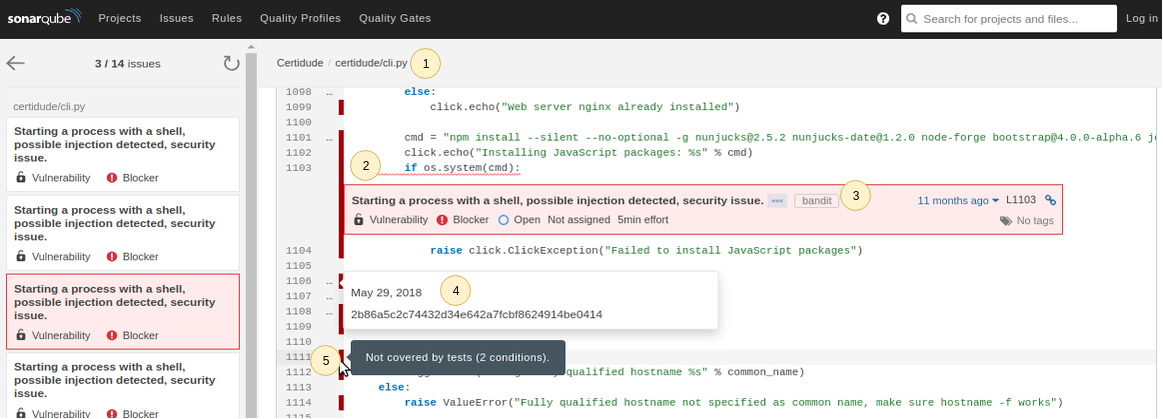
\includegraphics[width=1\linewidth]{figures/screenshots/sonarqube-analysis3.png}
    \end{minipage}
    \captionof{figure}{\textit{SonarQube: Code analysis and visualizations.}}
    \label{fig:sonarqube-result}
\end{figure}

An interesting feature that can also be observed in this pipeline is inheritance of instructions between tasks. This aims to clean up the pipeline file by reuse of the same code block through references instead of duplicating code. In Figure \ref{fig:yaml-anchor} one can see a reference (\textit{\&install-deps}) being created for a hidden task (\textit{.python-install-dependencies}). One can hide a task from being run by prepending a dot to the name of the task and will prevent it from being executed. In inheriting tasks (e.g. \textit{Pylint}) this "pointer" to the task is "de-referenced" (\textit{*install-deps}) which inserts the code block belonging to the task in its place.

\begin{figure}[H]
\centering
\begin{lstlisting}[frame=single, basicstyle=\small, linewidth=\textwidth]
.python-install-dependencies: &install-deps |-
  sudo apt-get update -qy
  ...
  
pylint:
  stage: test
  before_script:
    - *install-deps
  ...
\end{lstlisting}
\caption{\textit{Inheritance through YAML anchors in Gitlab configuration files.}}
\label{fig:yaml-anchor}
\end{figure}

\section{VirtualBox}\label{vbox-cert}
So far only a native shell build agent has been used, which means the agent fetches instructions from the CI/CD server and tries to execute any shell commands as the user that runs the agent. This is done in a temporary working directory created for that task. For Gitlab the default \textit{gitlab-runner} user is used which gets created when the agent is installed.\cite{gitlab-runner} In Gitlab terminology a build agent is also referred to as a runner and how this runner executes its fetched instructions is referred to as "\textit{executor}". A runner needs to be registered to the main CI/CD server, where it authenticates and indicates its executor type (e.g. Shell or VirtualBox), configuration options (e.g. name of VM or snapshot) and any associated tags. Multiple runners can be registered on the same machine using different executors. Tags are a way for the main CI/CD server to designate tasks to specific runners and/or executors. 

Best practice would be to have access to reusable virtual environments though and Gitlab integrates well with Docker and VirtualBox to provide these. While docker containers were previously used through shell commands (and have a nicer YAML syntax as well for docker executor), preference sometimes goes towards having full-fledged virtual machines available. This is also the case for Certidude, its tests and some of the components it needs to interact with.

Gitlab-runner was installed on the author's personal laptop which was connected over a VPN to the Gitlab CI instance.\cite{gitlab-runner} VirtualBox was installed, an Ubuntu 16.04 VM was created and OpenSSH server installed within, key based access was setup and the runner was registered to the Gitlab CI instance as a VirtualBox executor, pointing to the created VM. In addition the runner was also setup in the VM itself so as to allow for artifact uploads back to the CI/CD server. Several guides were used to do all this, including one provided by Gitlab.\cite{vbox-cli, vbox-oracle, gitlab-runner} All the steps that were performed are included in Appendix \hyperref[chapter:appendix-vbox]{8}. Using the executor is done transparently by simply including the registered tag for that executor in the defined pipeline task.

Figure \ref{fig:gitlab-runner-conf} shows the subsequent configuration file that was created in "\textit{/etc/gitlab-runner/config.toml}"

\pagebreak


\begin{figure}[H]
\centering
\begin{lstlisting}[frame=single, basicstyle=\small, linewidth=\textwidth]
[[runners]]
  name = "VirtualBox Runner"
  url = "https://<address/ip>/"
  token = "some-secret-shared-between-the-runner-and-server"
  executor = "virtualbox"
  [runners.custom_build_dir]
  [runners.ssh]
    user = "username"
    password = "password"
    identity_file = "/home/user/.ssh/id_rsa_vbox_runner"
  [runners.virtualbox]
    base_name = "Ubuntu-1604"
    disable_snapshots = false
  [runners.cache]
    [runners.cache.s3]
    [runners.cache.gcs]
\end{lstlisting}
\caption{\textit{Gitlab Virtualbox-Runner configuration file.}}
\label{fig:gitlab-runner-conf}
\end{figure}

\section{OpenWrt}\label{openwrt}

One request from supervisor and main developer of Certidude, \supervisor, was to have an OpenWrt image compilation step. OpenWrt is a Linux OS targeting embedded devices like routers.\cite{openwrt} The reason for this desire is to assist IOT (Internet Of Things) devices that don't support modern cryptographic libraries to still communicate over secure channels with the outside world. This would be done by transparently encrypting traffic through a VPN by the custom firmware image created which would be flashed on a small router placed between the device and the outside world. In this scenario Certidude would be the tool to help orchestrate and manage any certificate signing and validation. 

Appendix \hyperref[chapter:appendix-openwrt]{9} shows the created pipeline step to produce a custom OpenWrt image. The actual image customization has been left out, but would be integrated in the script-part of the \textit{build\_image} job.\cite{openwrt-build} This step extends Continuous Integration into Continuous Delivery for Certidude by producing a production ready router image. It shows how artifact creation and possible deployment steps are a natural extension of the CI development practice. 

\pagebreak

\section{Future Work} \label{future-work}
Future work involves dissecting, correcting and expanding the current test suite of Certidude which is not passing at the moment of this writing. Some of the current tests assume behavior no longer present in the code base while other code has been altered enough to break the tests (e.g. structure of API calls). The following list contains some concrete suggestions for future improvement.

\begin{itemize}
    \item The current setup of Gitlab and SonarQube are private but could instead be moved to a dedicated public facing address. SSL (Secure Sockets Layer) / TLS (Transport Layer Security) certificates need to be setup and SonarQube needs to be properly installed alongside some supporting database solution.
    \item The current test suite contains a complex sequence of services being provisioned to test integration with Certidude. These services include a Samba DC, OpenVPN / StrongSwan clients and gateways. The provisioning of these services lend themselves perfectly for both parallelization as well as virtualization. This would mean launching various containers and virtual machines at the same time providing these services. This is now possible.
    \item More integration tests for FreeBSD, Juniper, Cisco and Windows. This would involve expanding on the VM runner integration of Gitlab CI. Perhaps a GNS3 VM could potentially be used to simulate complex network scenarios with Cisco or using Junos OS based vMX virtual router. There is also Docker for Windows available which was not explored in this work.
    \item More CD pipeline steps to build and deploy code. This could include integration with a configuration management system like Chef, Puppet or Ansible as well as package creation (e.g. pip).
    \item Expand the integration test suite by including Selenium. This would require a build step where Certidude gets fully built and run.  
    \item Expand on the security test suite by putting tools like OWASP ZAP between the integration tests written with Selenium and the Certidude instance or use clair to perform container vulnerability scans. At the moment of this writing there is an attempt being made to properly containerize Certidude which would make this last addition more relevant.
\end{itemize}








\pagebreak
\pagebreak



\iffalse % Starts dummy text

\begin{itemize}
    \item Deconstruct Certidude here a bit
    \item Deconstruct its tests; this is quite hard at the moment since they are not up-to-date
    \item 
\end{itemize}


* Dockerfiles for OpenVPN / StrongSwan / WireGuard
Alpine vs. Centos vs. Ubuntu..?


% This is might be because of defaul EE edition, no bronze/gold/ultimate.. this could be requested? 
% I suspect it just needs formatting
* pylint reports can be generated in json format, but gitlabci expects these to be in predefined format 
\url{https://docs.gitlab.com/ee/user/project/merge_requests/code_quality.html}
\url{https://docs.gitlab.com/ee/user/project/pipelines/job_artifacts.html}
\url{https://docs.pylint.org/en/1.6.0/output.html}
\url{https://realpython.com/python-json/}
Upload of artifacts fails using artififacts:reports:junit / codequality etc. Normal upload works. 
Maybe try to convert pylint report into right format anyways? Also for bandit?
pylint --output-format=json example/ >> pylint1.json 

* Describe sonarube install? \url{https://docs.sonarqube.org/latest/setup/get-started-2-minutes/}
  See for scanner install: \url{https://docs.sonarqube.org/display/SCAN/Analyzing+with+SonarQube+Scanner}
  Then see about sonarpython \url{https://docs.sonarqube.org/display/PLUG/SonarPython}
 
 - docker pull sonarqube:latest
   docker run -d --name sonarqube -p 9000:9000 sonarqube
 - Download / Install:  \url{https://binaries.sonarsource.com/Distribution/sonar-scanner-cli/sonar-scanner-cli-3.3.0.1492-linux.zip}
 
 - Setting the sonar.python.coverage.reportPaths variable in home directory config file to point to coverage file..
 - login as admin/admin -> administration -> marketplace -> python this way you can also install the sonarpyhton plugin
 - login as admin/admin -> Quality Profiles -> should show the python one, but a lot of rules are deactivated
   -> bulk change and activate all (non-depricated) rules -> back to quality profiles and set new one as default..
 - \url{https://docs.sonarqube.org/latest/analysis/analysis-parameters/}
 - atm link back to source code files is not present in junit test reports, so it will only show that there are x failing tests..
   \url{https://stackoverflow.com/questions/29117785/no-drilldown-from-sonarqube-unit-test-success-widget}
   
 - set .profile to include solar-scanner/bin as part of PATH for gitlab-runner user..
 
\fi % Ends dummy text

\chapter{Summary}\label{chapter:summary} 
When developers write software and want to properly test, build and deploy their code they can spend a lot of time on manual tasks to do so. Continuous Integration and Continuous Delivery practices aim to automate these best practices through the use of automation servers. This should ensure code is tested as much as possible while reducing the amount of time spent on performing manual tasks as well as reduce the number of mistakes made during execution. They enforce that these steps are actually performed and increase confidence in the secure and proper functionality of the code itself.

This thesis compared and analyzed various popular CI/CD servers, integrations and their suitability for Certidude to see what solution could replace the one currently in use. This was also done to relieve fundamental complaints of the current tool, continue to be able to automatically run tests as well as improve and expand on the defined pipeline. These alternative solutions were explored, tested and compared by using a dummy application developed by the author for this thesis and writing pipeline definitions for each one of these tools. Gitlab CI was found to be the most relevant CI/CD server to Certidude by both the comparative analysis as by the main developer of Certidude, \supervisor.

This thesis contributed a working replacement installation and pipeline for the current CI/CD setup in use as well as an expansion on functionality by the inclusion of multiple static code analysis tasks and an OpenWrt image creation task in the developed pipeline. A list of "future work" suggestions was compiled which can be used as part of a development road map for Certidude.

\pagebreak
\phantomsection
\addcontentsline{toc}{chapter}{Bibliography}
\printbibliography

\pagebreak

\phantomsection
\appendix
\addcontentsline{toc}{chapter}{Appendices}
\chapter*{Appendices}
\renewcommand{\thechapter}{\arabic{chapter}}

\addcontentsline{toc}{chapter}{Appendix 1 - Test Pipeline - Travis CI}\label{chapter:appendix-travis}
{\let\clearpage\relax\chapter*{Appendix 1 - Test Pipeline - Travis CI}}
\begin{lstlisting}[frame=single, basicstyle=\tiny]
language: generic
cache: pip
dist: xenial

env:
  global:
    - TEST_NAME="thesis-cicd-poc"

jobs:
  include:
    - stage: build-run-test
      name: "Installing dependencies and building docker image"
      script:
        - sudo apt-get update -qy
        - sudo apt-get install -y python3-dev python3-pip
        - sudo -H pip3 install pytest
        - docker build -t $TEST_NAME .
        - docker run -dt -p 8282:80 -v $PWD:/tmp/ --name travisCICDContainer $TEST_NAME
        - pytest tests/

    - stage: test
      name: "Running functional tests with fixtures"
      script:
        - sudo apt-get update -qy
        - sudo apt-get install -y python3-dev python3-pip
        - sudo -H pip3 install -U pytest-cov pytest codecov
        - sudo -H pip3 install -r requirements.txt
        - pytest tests2/
        - pytest --cov-report term --cov-branch --cov=example/ tests2/
      after_success:
        - codecov

    - stage: deploy
      name: "Simulating a deployment step"
      script:
        - echo "Deploying..."

stages:
  - build-run-test
  - test
  - name: deploy
    if: branch = master

notifications:
  email:
    on_success: never
    on_failure: always
\end{lstlisting}


\clearpage
\phantomsection
\addcontentsline{toc}{chapter}{Appendix 2 - Test Pipeline - Jenkins}\label{chapter:appendix-jenkins}
\chapter*{Appendix 2 - Test Pipeline - Jenkins}
\begin{lstlisting}[frame=single, basicstyle=\tiny]
pipeline {
  agent any
  environment {
    CNAME = "jenkins-cicd-container-$GIT_COMMIT"
  }
  stages {
    stage('Build') {
      steps {
        echo 'Building..'
        sh "docker build -t $CNAME ."
      }
    }
    stage('Run') {
      steps {
        echo 'Running appliances'
        sh '''docker kill $(docker ps -q) || true
              docker rm $(docker ps -a -q) || true
              docker run -dt -p 8282:80 -v $PWD:/tmp/ --name jenkinsCICDContainer $CNAME'''
      }
    }
    stage('Test') {
      steps {
        echo 'Testing...'
        sh '''sudo apt-get update -qy
	      sudo apt-get install -y python3-dev python3-pip
	      sudo pip3 install pytest pytest-cov
	      pytest --cov-report xml --cov-report term --cov-branch --cov=example/ tests/'''
      }
    }
    stage('Deploy') {
      when {
        expression {
	  currentBuild.result == null || currentBuild.result == 'SUCCESS'
	}
      }
      steps {
        echo 'Deploying...'
      }
    }
    stage('Clean') {
      steps {
        echo 'Cleaning up...'
        sh '''docker kill $(docker ps -q) || true
	      docker rm $(docker ps -a -q) || true'''
      }
    }
  }
}
\end{lstlisting}


\clearpage
\phantomsection
\addcontentsline{toc}{chapter}{Appendix 3 - Test Pipeline - Gitlab CI}\label{chapter:appendix-gitlab}
\chapter*{Appendix 3 - Test Pipeline - Gitlab CI}

\begin{lstlisting}[frame=single, basicstyle=\tiny]
variables:
  TEST_NAME: 172.20.8.193:5001/thesis-examples/thesis-cicd-poc:$CI_COMMIT_REF_NAME

stages:
  - build
  - run
  - test
  - clean

build_docker_image:
  stage: build
  script:
    - docker login -u $REG_UNAME -p $REG_PASSWORD $REG_TARGET 
    - docker build -t $TEST_NAME .
    - docker push $TEST_NAME
  tags:
    - build

run_docker_image:
  stage: run
  script:
    - docker login -u $REG_UNAME -p $REG_PASSWORD $REG_TARGET
    - docker pull $TEST_NAME
    - docker run -dt -p 8282:80 -v $PWD:/tmp/ --name gitlabCICDContainer $TEST_NAME
  tags:
    - run

test_project:
  stage: test
  script:
    - sudo apt-get update -qy
    - sudo apt-get install -y python3-dev python3-pip
    - sudo pip3 install pytest pytest-cov
    - pytest --cov=example/ tests/
  tags:
    - test

test_project_with_fixtures:
  stage: test
  script:
  - pytest --junitxml=$CI_PROJECT_PATH/TEST_RESULTS.xml --cov-report xml \
                    --cov-report term --cov-branch --cov=example/ tests2/
  artifacts:
    reports:
      junit: $CI_PROJECT_PATH/TEST_RESULTS.xml
  tags:
    - test

clean_docker_images:
  stage: clean
  script:
    - docker kill $(docker ps -q) || true
    - docker rm $(docker ps -a -q) || true
  tags:
    - clean
\end{lstlisting}



\clearpage
\phantomsection
\addcontentsline{toc}{chapter}{Appendix 4 - Test Pipeline - TeamCity}\label{chapter:appendix-tc}
\chapter*{Appendix 4 - Test Pipeline - TeamCity}
\begin{lstlisting}[frame=single, basicstyle=\tiny]
package _Self.buildTypes
import jetbrains.buildServer.configs.kotlin.v2018_2.*
import jetbrains.buildServer.configs.kotlin.v2018_2.buildSteps.script
import jetbrains.buildServer.configs.kotlin.v2018_2.triggers.vcs

object Build : BuildType({
    name = "Thesis-Example-Pipeline"

    vcs {
        root(Git172208193thesisExamplesThesisCicdPocGitRefsHeadsMaster)
    }
steps {
    script {
        name = "Build"
        scriptContent = """
            echo 'Building..'
            docker build -t teamcity-cicd-container-${'$'}BUILD_VCS_NUMBER .
        """.trimIndent()
    }
    script {
        name = "Run"
        scriptContent = """
            echo 'Running..'
            docker kill ${'$'}(docker ps -q) || true
            docker rm ${'$'}(docker ps -a -q) || true
            docker run -dt -p 8282:80 -v ${'$'}PWD:/tmp/ --name teamcityCICDContainer \
                                        teamcity-cicd-container-${'$'}BUILD_VCS_NUMBER
        """.trimIndent()
    }
    script {
        name = "Test"
        scriptContent = """
            echo 'Testing...'
            sudo apt-get update -qy
            sudo apt-get install -y python3-dev python3-pip
            sudo pip3 install pytest pytest-cov teamcity-messages
            pytest --teamcity --cov-branch --cov=example/ tests/
        """.trimIndent()
    }
    script {
        name = "Clean"
        scriptContent = """
            echo 'Cleaning up...'
            docker kill ${'$'}(docker ps -q) || true
            docker rm ${'$'}(docker ps -a -q) || true
        """.trimIndent()
    }
}
    triggers {
        vcs {
        }
    }
})
\end{lstlisting}


\clearpage
\phantomsection
\addcontentsline{toc}{chapter}{Appendix 5 - Test Pipeline - Circle CI}\label{chapter:appendix-circleci}
\chapter*{Appendix 5 - Test Pipeline - Circle CI}
\begin{lstlisting}[frame=single, basicstyle=\tiny]
workflows:
  version: 2
  build-deploy:
    jobs:
      - build
      - build-fixtures
      - deploy:
          requires:
            - build
            - build-fixtures
          filters:
            branches:
             only: master

version: 2
jobs:
  build:
    machine:
      image: ubuntu-1604:201903-01
    environment:
      TEST_NAME: thesis-cicd-poc
    steps:
      - restore_cache:
          key: v1-source-{{ .Branch }}-{{ .Revision }}
      - checkout
      - save_cache:
          key: v1-source-{{ .Branch }}-{{ .Revision }}
          paths:
            - ".git"
      - run:
          name: Environment Discovery
          command: |
            whoami
            ifconfig
            lsb_release -a
      - run:
          name: Installing dependencies
          command: |
            sudo apt-get update -qy
            sudo apt-get install -y python3-dev python3-pip
            sudo -H pip3 install pytest
      - run:
          name: Setting up Docker
          command: |
            docker build -t $TEST_NAME .
            docker run -dt -p 8282:80 -v $PWD:/tmp/ --name circleCICDContainer $TEST_NAME
      - run:
          name: Running Tests
          command: |
            pytest tests/
  build-fixtures:
    machine:
      image: ubuntu-1604:201903-01
    steps:
      - checkout
      - run:
          name: Installing dependencies
          command: |
            sudo apt-get update -qy
            sudo apt-get install -y python3-dev python3-pip
            sudo -H pip3 install -U pytest-cov pytest codecov
            sudo -H pip3 install -r requirements.txt
      - run:
          name: Running tests using fixtures
          command: |
            pytest --junitxml=$PWD/test-results/test-results.xml --cov-report term \
                                                --cov-branch --cov=example/ tests2/
      - store_test_results:
          path: test-results

  deploy:
    docker:
      - image: circleci/python:3.5
    steps:
      - checkout
      - setup_remote_docker:
          docker_layer_caching: true
      - run: docker build .
      - run:
          name: Dummy deploy somewhere
          command: 
            echo "Deploying..."
\end{lstlisting}

\clearpage
\phantomsection
\addcontentsline{toc}{chapter}{Appendix 6 - Certidude Pipeline}\label{chapter:appendix-certidude-pipeline}
\chapter*{Appendix 6 - Certidude Pipeline}
\begin{lstlisting}[frame=single, basicstyle=\tiny]
---

variables:
  SONARQUBE: 172.20.8.193:5001/certidude/certidude:sonarqube

stages:
  - build
  - test
  - scan

.python-install-dependencies: &install-deps |-
  sudo apt-get update -qy
  sudo apt-get install -y python3-dev python3-pip
  sudo pip3 install pylint
  sudo pip3 install pytest pytest-cov
  sudo pip3 install bandit

pylint:
  stage: test
  allow_failure: true
  before_script:
    - *install-deps
  script:
    - pylint --output-format=json certidude/ > pylint-results.json || true
  artifacts:
    paths:
      - "pylint-results.json"
    expire_in: 2 years
  tags:
    - main

pytest:
  stage: test
  allow_failure: true
  before_script:
    - *install-deps
  script:
    - sudo -H pip3 install -r requirements.txt
    - pytest --junitxml=test_results.xml --cov-report xml --cov-report term --cov-branch --cov=certidude/ tests/ || true
  artifacts:
    paths:
      - "test_results.xml"
      - "coverage.xml"
    expire_in: 2 years
  tags:
    - main

bandit:
  stage: test
  allow_failure: true
  before_script:
    - *install-deps
  script:
    - bandit --format json --output bandit-report.json --recursive certidude/ || true
    - bandit -r certidude/ --format xml --output bandit_results.xml || true
  artifacts:
    paths:
      - bandit_results.xml
      - bandit-report.json
    expire_in: 2 years
  tags:
    - main

sonar_docker:
  stage: build
  script:
    - docker login -u $REG_UNAME -p $REG_PASSWORD $REG_TARGET
    - docker pull $SONARQUBE
    - docker run -d -p 9000:9000 $SONARQUBE || true
  tags:
    - sonar

sonar_scanner:
  stage: scan
  allow_failure: true
  script:
    - wget https://binaries.sonarsource.com/Distribution/sonar-scanner-cli/sonar-scanner-cli-3.3.0.1492-linux.zip
    - mkdir sonar-scanner
    - unzip sonar-scanner-cli-*-linux.zip -d sonar-scanner
    - mv sonar-scanner/*/* sonar-scanner/
    - export PATH=$(pwd)/sonar-scanner/bin:$PATH
    - sonar-scanner
  dependencies:
    - bandit
    - pytest
    - pylint
  tags:
    - sonar
\end{lstlisting}

\phantomsection
\addcontentsline{toc}{chapter}{Appendix 7 - SonarScanner Configuration}\label{chapter:appendix-sonar}
{\let\clearpage\relax\chapter*{Appendix 7 - SonarScanner Configuration}}
\begin{lstlisting}[frame=single, basicstyle=\tiny]
sonar.host.url=http://localhost:9000
sonar.projectKey=certidude:sonar
sonar.projectName=Certidude
sonar.projectVersion=1.0

# Point to certidude code
sonar.sources=./certidude/

# Point to coverage report generated by pytest
sonar.python.coverage.reportPaths=coverage.xml            

# Point to json bandit report
sonar.python.bandit.reportPaths=bandit-report.json

# Point to xunit file generated by pytest
sonar.python.xunit.reportPath=test_results.xml            

# Point to test dir
sonar.tests=./tests/
\end{lstlisting}

\clearpage
\phantomsection
\addcontentsline{toc}{chapter}{Appendix 8 - VirtualBox Executor}\label{chapter:appendix-vbox}
\chapter*{Appendix 8 - VirtualBox Executor}
\begin{lstlisting}[frame=single, basicstyle=\tiny]
# Download the desired OS flavor iso
wget http://releases.ubuntu.com/16.04/ubuntu-16.04.6-server-amd64.iso

# Set the VM Name
VM='Ubuntu-1604'

# Create the Virtual Disk Image file for storage
VBoxManage createhd         --filename $VM.vdi --size 32768

# Create the Ubuntu x64 VM
VBoxManage createvm         --name $VM --ostype Ubuntu_64 --register

# Create and attach the SATA controller with the previous HD
VBoxManage storagectl       $VM --name "SATA Controller" --add sata --controller IntelAHCI
VBoxManage storageattach    $VM --storagectl "SATA Controller" --port 0 --device 0 --type hdd --medium $VM.vdi

# Create IDE controller and insert the downloaded OS image
VBoxManage storagectl       $VM --name "IDE Controller" --add ide
VBoxManage storageattach    $VM --storagectl "IDE Controller" --port 0 --device 0 --type dvddrive \\
                                --medium ubuntu-16.04.6-server-amd64.iso
    
# Attach needed Memory to the VM
VBoxManage modifyvm         $VM --memory 2048

# Create and add 2 Network Interfaces. The first is required to be NAT by Gitlab CI.
VBoxManage modifyvm         $VM --nic1 nat
VBoxManage modifyvm         $VM --bridgeadapter1 vmnet1
VBoxManage modifyvm         $VM --nic2 bridged

# Start the VM either directly or in headless mode
VBoxManage startvm $VM
VBoxHeadless -s $VM

# Setup VNC to manage the installation of the OS remotely
VBoxManage          setproperty vrdeextpack VNC
VBoxManage          modifyvm $VM --vrdeproperty VNCPassword=<password>
VBoxHeadless        --vrde on -s $VM

sudo apt install vncviewer
vncviewer 0.0.0.0:3389
vncviewer -encodings tight 0.0.0.0:3389  # Needed when encoding doesn't match

# Or alternatively if VRDE is working:
VBoxManage modifyvm $VM --vrde on
rdesktop -a 16 -N 127.0.0.1:3389

# To shutdown the VM
VBoxManage          controlvm $VM poweroff soft
VBoxManage          controlvm $VM acpipowerbutton

# To take a snapshot of the machine (name can be included during Gitlab registration process)
VBoxManage          snapshot $VM take example-snapshot-name


# Gitlab Runner Installation. Needed both on the guest and host machines.
sudo wget -O /usr/local/bin/gitlab-runner \\
             https://gitlab-runner-downloads.s3.amazonaws.com/latest/binaries/gitlab-runner-linux-amd64
sudo chmod +x /usr/local/bin/gitlab-runner
curl -sSL https://get.docker.com/ | sh
sudo useradd --comment 'GitLab Runner' --create-home gitlab-runner --shell /bin/bash
sudo gitlab-runner install --user=gitlab-runner --working-directory=/home/gitlab-runner
sudo gitlab-runner start


# The following dumped the initial self-signed pem-encoded certificate of the Gitlab CI instance.
echo | openssl x509 -in <(openssl s_client -connect <ip/hostname>:443 -prexit 2>/dev/null) > cert.pem

# Moves the certificate to list of trusted hosts. Certificates are now trusted so that API calls succeed.
mv cert.pem /etc/gitlab-runner/certs/<ip/hostname>.crt


# Gitlab Executor can now be setup from the host machine.
gitlab-runner register
Runtime platform                    arch=amd64 os=linux pid=20151 revision=3001a600 version=11.10.0
Running in system-mode.
                            
Please enter the gitlab-ci coordinator URL (e.g. https://gitlab.com/):
https://<ip/hostname>/
Please enter the gitlab-ci token for this runner:
<API Token retrieved from Gitlab CI UI>
Please enter the gitlab-ci description for this runner:
VirtualBox Runner
Please enter the gitlab-ci tags for this runner (comma separated):
vbox-ubunutu16
Registering runner... succeeded     runner=<uid>
Please enter the executor: parallels, docker+machine, virtualbox, docker-ssh+machine, \\
                           kubernetes, docker, docker-ssh, shell, ssh:
virtualbox
Please enter the VirtualBox VM (e.g. my-vm):
Ubuntu-1604
Please enter the SSH user (e.g. root):
<user>
Please enter the SSH password (e.g. docker.io):
<password>
Please enter path to SSH identity file (e.g. /home/user/.ssh/id_rsa):
<path/to/identityfile>
Runner registered successfully. Feel free to start it, but if it's running already the config \\
                                should be automatically reloaded! 
\end{lstlisting}

\clearpage
\phantomsection
\addcontentsline{toc}{chapter}{Appendix 9 - OpenWrt Image Creation Pipeline}\label{chapter:appendix-openwrt}
\chapter*{Appendix 9 - OpenWrt Image Creation Pipeline}
\begin{lstlisting}[frame=single, basicstyle=\tiny]
---

variables:
  IMAGE_PATH: 'bin/targets/ramips/mt76x8/openwrt-ramips-mt76x8-gl-mt300n-v2-squashfs-sysupgrade.bin'
  IMAGE_PATH_GLOB: 'bin/targets/*/*/*.bin'

stages:
  - init
  - build

install_dependencies:
  stage: init
  script:
    - sudo apt install -y subversion g++ zlib1g-dev build-essential git python time
    - sudo apt install -y libncurses5-dev gawk gettext unzip file libssl-dev wget
    - sudo apt install -y libelf-dev
  tags:
    - openwrt

build_image:
  stage: build
  script:
    - git clone https://git.openwrt.org/openwrt/openwrt.git
    - cp .config openwrt/
    - cd openwrt
    - echo "=================================================="
    - echo "==== Apply patch / run builder scripts here  ====="
    - echo "=================================================="
    - ./scripts/feeds update -a
    - ./scripts/feeds install -a
    - ./scripts/diffconfig.sh > configdiff
    - cp configdiff .config
    - make defconfig;make oldconfig
    - make download
    - make -j128
    - cp $IMAGE_PATH .
  artifacts:
    paths:
      - "*.bin"
    expire_in: 1 year
  when: manual
  tags:
    - openwrt

\end{lstlisting}

\end{document}